\documentclass[]{article}
\usepackage{lmodern}
\usepackage{amssymb,amsmath}
\usepackage{ifxetex,ifluatex}
\usepackage{bm}
\usepackage{soul}
\usepackage[color=yellow]{todonotes}
\usepackage{fixltx2e} % provides \textsubscript
\ifnum 0\ifxetex 1\fi\ifluatex 1\fi=0 % if pdftex
  \usepackage[T1]{fontenc}
  \usepackage[utf8]{inputenc}
\else % if luatex or xelatex
  \ifxetex
    \usepackage{mathspec}
  \else
    \usepackage{fontspec}
  \fi
  \defaultfontfeatures{Ligatures=TeX,Scale=MatchLowercase}
\fi
% use upquote if available, for straight quotes in verbatim environments
\IfFileExists{upquote.sty}{\usepackage{upquote}}{}
% use microtype if available
\IfFileExists{microtype.sty}{%
\usepackage{microtype}
\UseMicrotypeSet[protrusion]{basicmath} % disable protrusion for tt fonts
}{}
\usepackage[margin=1in]{geometry}
\usepackage{hyperref}
\hypersetup{unicode=true,
            pdftitle={10 Statistical methodology for nonlinear partially observed Markov process models},
            pdfauthor={Edward Ionides},
            pdfborder={0 0 0},
            breaklinks=true}
\urlstyle{same}  % don't use monospace font for urls
\usepackage{color}
\usepackage{fancyvrb}
\newcommand{\VerbBar}{|}
\newcommand{\VERB}{\Verb[commandchars=\\\{\}]}
\DefineVerbatimEnvironment{Highlighting}{Verbatim}{commandchars=\\\{\}}
% Add ',fontsize=\small' for more characters per line
\usepackage{framed}
\definecolor{shadecolor}{RGB}{248,248,248}
\newenvironment{Shaded}{\begin{snugshade}}{\end{snugshade}}
\newcommand{\KeywordTok}[1]{\textcolor[rgb]{0.13,0.29,0.53}{\textbf{#1}}}
\newcommand{\DataTypeTok}[1]{\textcolor[rgb]{0.13,0.29,0.53}{#1}}
\newcommand{\DecValTok}[1]{\textcolor[rgb]{0.00,0.00,0.81}{#1}}
\newcommand{\BaseNTok}[1]{\textcolor[rgb]{0.00,0.00,0.81}{#1}}
\newcommand{\FloatTok}[1]{\textcolor[rgb]{0.00,0.00,0.81}{#1}}
\newcommand{\ConstantTok}[1]{\textcolor[rgb]{0.00,0.00,0.00}{#1}}
\newcommand{\CharTok}[1]{\textcolor[rgb]{0.31,0.60,0.02}{#1}}
\newcommand{\SpecialCharTok}[1]{\textcolor[rgb]{0.00,0.00,0.00}{#1}}
\newcommand{\StringTok}[1]{\textcolor[rgb]{0.31,0.60,0.02}{#1}}
\newcommand{\VerbatimStringTok}[1]{\textcolor[rgb]{0.31,0.60,0.02}{#1}}
\newcommand{\SpecialStringTok}[1]{\textcolor[rgb]{0.31,0.60,0.02}{#1}}
\newcommand{\ImportTok}[1]{#1}
\newcommand{\CommentTok}[1]{\textcolor[rgb]{0.56,0.35,0.01}{\textit{#1}}}
\newcommand{\DocumentationTok}[1]{\textcolor[rgb]{0.56,0.35,0.01}{\textbf{\textit{#1}}}}
\newcommand{\AnnotationTok}[1]{\textcolor[rgb]{0.56,0.35,0.01}{\textbf{\textit{#1}}}}
\newcommand{\CommentVarTok}[1]{\textcolor[rgb]{0.56,0.35,0.01}{\textbf{\textit{#1}}}}
\newcommand{\OtherTok}[1]{\textcolor[rgb]{0.56,0.35,0.01}{#1}}
\newcommand{\FunctionTok}[1]{\textcolor[rgb]{0.00,0.00,0.00}{#1}}
\newcommand{\VariableTok}[1]{\textcolor[rgb]{0.00,0.00,0.00}{#1}}
\newcommand{\ControlFlowTok}[1]{\textcolor[rgb]{0.13,0.29,0.53}{\textbf{#1}}}
\newcommand{\OperatorTok}[1]{\textcolor[rgb]{0.81,0.36,0.00}{\textbf{#1}}}
\newcommand{\BuiltInTok}[1]{#1}
\newcommand{\ExtensionTok}[1]{#1}
\newcommand{\PreprocessorTok}[1]{\textcolor[rgb]{0.56,0.35,0.01}{\textit{#1}}}
\newcommand{\AttributeTok}[1]{\textcolor[rgb]{0.77,0.63,0.00}{#1}}
\newcommand{\RegionMarkerTok}[1]{#1}
\newcommand{\InformationTok}[1]{\textcolor[rgb]{0.56,0.35,0.01}{\textbf{\textit{#1}}}}
\newcommand{\WarningTok}[1]{\textcolor[rgb]{0.56,0.35,0.01}{\textbf{\textit{#1}}}}
\newcommand{\AlertTok}[1]{\textcolor[rgb]{0.94,0.16,0.16}{#1}}
\newcommand{\ErrorTok}[1]{\textcolor[rgb]{0.64,0.00,0.00}{\textbf{#1}}}
\newcommand{\NormalTok}[1]{#1}
\usepackage{graphicx,grffile}
\makeatletter
\def\maxwidth{\ifdim\Gin@nat@width>\linewidth\linewidth\else\Gin@nat@width\fi}
\def\maxheight{\ifdim\Gin@nat@height>\textheight\textheight\else\Gin@nat@height\fi}
\makeatother
% Scale images if necessary, so that they will not overflow the page
% margins by default, and it is still possible to overwrite the defaults
% using explicit options in \includegraphics[width, height, ...]{}
\setkeys{Gin}{width=\maxwidth,height=\maxheight,keepaspectratio}
\IfFileExists{parskip.sty}{%
\usepackage{parskip}
}{% else
\setlength{\parindent}{0pt}
\setlength{\parskip}{6pt plus 2pt minus 1pt}
}
\setlength{\emergencystretch}{3em}  % prevent overfull lines
\providecommand{\tightlist}{%
  \setlength{\itemsep}{0pt}\setlength{\parskip}{0pt}}
%\setcounter{secnumdepth}{0}
\setcounter{section}{10}
% Redefines (sub)paragraphs to behave more like sections
\ifx\paragraph\undefined\else
\let\oldparagraph\paragraph
\renewcommand{\paragraph}[1]{\oldparagraph{#1}\mbox{}}
\fi
\ifx\subparagraph\undefined\else
\let\oldsubparagraph\subparagraph
\renewcommand{\subparagraph}[1]{\oldsubparagraph{#1}\mbox{}}
\fi

%%% Use protect on footnotes to avoid problems with footnotes in titles
\let\rmarkdownfootnote\footnote%
\def\footnote{\protect\rmarkdownfootnote}

%%% Change title format to be more compact
\usepackage{titling}

% Create subtitle command for use in maketitle
\newcommand{\subtitle}[1]{
  \posttitle{
    \begin{center}\large#1\end{center}
    }
}

\setlength{\droptitle}{-2em}
  \title{10. Statistical methodology for nonlinear partially observed Markov
process models}
  \pretitle{\vspace{\droptitle}\centering\huge}
  \posttitle{\par}
  \author{Edward Ionides}
  \preauthor{\centering\large\emph}
  \postauthor{\par}
  \predate{\centering\large\emph}
  \postdate{\par}
  \date{3/12/2018}


\begin{document}
\maketitle

{
\setcounter{tocdepth}{2}
\tableofcontents
}
\newcommand\prob{\mathbb{P}}
\newcommand\E{\mathbb{E}}
\newcommand\var{\mathrm{Var}}
\newcommand\cov{\mathrm{Cov}}
\newcommand\loglik{\ell}
\newcommand\R{\mathbb{R}}
\newcommand\data[1]{#1^*}
\newcommand\params{\, ; \,}
\newcommand\transpose{\scriptsize{T}}
\newcommand\eqspace{\quad\quad}
\newcommand\myeq[1]{\eqspace \displaystyle #1}
\newcommand\lik{\mathscr{L}}
\newcommand\profileloglik[1]{\ell^\mathrm{profile}_#1}
\newcommand\ar{\phi}
\newcommand\ma{\psi}
\newcommand\AR{\Phi}
\newcommand\MA{\Psi}
\newcommand\ev{u}
\newcommand\given{{\, | \,}}
\newcommand\equals{{=\,}}
\newcommand\matA{\mathbb{A}}
\newcommand\matB{\mathbb{B}}
\newcommand\matH{\mathbb{H}}
\newcommand\covmatX{\mathbb{U}}
\newcommand\covmatY{\mathbb{V}}





\begin{center}\rule{0.5\linewidth}{\linethickness}\end{center}

\begin{center}\rule{0.5\linewidth}{\linethickness}\end{center}

Objectives

\begin{enumerate}
\def\labelenumi{\arabic{enumi}.}
\item
  To introduce students to the \textbf{pomp} package
\item
  To explain how the components of a POMP model are encoded in this
  package
\item
  To give some experience in the use and manipulation of \texttt{pomp}
  objects
\end{enumerate}

\begin{center}\rule{0.5\linewidth}{\linethickness}\end{center}

\begin{center}\rule{0.5\linewidth}{\linethickness}\end{center}

\subsection{Time series analysis via nonlinear partially observed Markov
process (NL-POMP)
models}\label{time-series-analysis-via-nonlinear-partially-observed-markov-process-nl-pomp-models}

\subsubsection{\texorpdfstring{Six problems of
\href{http://dx.doi.org/10.1126/science.1062226}{Bjornstad and Grenfell
(Science,
2001)}}{Six problems of Bjornstad and Grenfell (Science, 2001)}}\label{six-problems-of-bjornstad-and-grenfell-science-2001}

\begin{itemize}
\tightlist
\item
  Obstacles for \textbf{ecological} modeling and inference via nonlinear
  mechanistic models:
\end{itemize}

\begin{enumerate}
\def\labelenumi{\arabic{enumi}.}
\item
  Combining measurement noise and process noise.
\item
  Including covariates in mechanistically plausible ways.
\item
  Continuous time models.
\item
  Modeling and estimating interactions in coupled systems.
\item
  Dealing with unobserved variables.
\item
  Modeling spatial-temporal dynamics.
\end{enumerate}

\begin{center}\rule{0.5\linewidth}{\linethickness}\end{center}

\begin{center}\rule{0.5\linewidth}{\linethickness}\end{center}

\subsubsection{Applications of NL-POMP
models}\label{applications-of-nl-pomp-models}

\begin{itemize}
\item
  The same issues arise for any modeling and inference via nonlinear
  mechanistic models. This arises throughout engineering, the sciences
  (social, biological and physical) and business.
\item
  For example, in finance, we considered a stochastic volatility example
  in
  \href{http://ionides.github.io/531w16/notes01/intro.html\#models-dynamic-systems-state-space-models}{Chapter
  1}
\item
  Many applications arise in epidemiology, studying the transmission of
  infectious diseases.
\item
  Infectious disease dynamics can be highly nonlinear:

  \begin{enumerate}
  \def\labelenumi{\arabic{enumi}.}
  \item
    Transmission arises when an infected individual contacts a
    susceptible individual. This leads to a quadratic term in the rate
    of infections, which should be proportional to \[\begin{array}{ll}
    \mbox{Fraction of individuals infected}\\
    \quad\times\quad \mbox{Fraction of individuals susceptible to infection}
    \end{array}\]
  \item
    Each new infection depletes the pool of susceptible individuals.
  \item
    Without depletion of susceptibles, the fraction of individuals
    susceptible to infection is constant and the epidemic grows
    exponentially. Then, the system is linear on a log scale.
  \end{enumerate}
\item
  Data on infectious diseases are generally limited to diagnosed cases.
  Much of the transmission dynamics cannot be directly observed.
\item
  Infectious disease epidemiology has motivated developments in
  statistical methodology and software for NL-POMP models, including
  \href{http://kingaa.github.io/sbied/}{a previous course} used as a
  source for these class notes.
\item
  Many other biological populations have similar nonlinearities: the
  population grows exponentially until limited by some constraint (which
  could be a food resource or a predator). When the resource is used up,
  or the predator becomes abundant, the population crashes. Then a new
  cycle begins.
\end{itemize}

\begin{center}\rule{0.5\linewidth}{\linethickness}\end{center}

\begin{center}\rule{0.5\linewidth}{\linethickness}\end{center}

\subsection{An algorithmic approach to inference for POMP
models}\label{an-algorithmic-approach-to-inference-for-pomp-models}

\begin{itemize}
\item
  Recall our notation for partially observed Markov process models.
\item
  Write \(X_n=X(t_n)\) and \(X_{0:N}=(X_0,\dots,X_N)\). Let \(Y_n\) be a
  random variable modeling the observation at time \(t_n\).
\item
  The one-step transition density,
  \(f_{X_n|X_{n-1}}(x_n|x_{n-1};\theta)\), together with the measurement
  density, \(f_{Y_n|X_n}(y_n|x_n;\theta)\) and the initial density,
  \(f_{X_0}(x_0;\theta)\), specify the entire joint density via
\end{itemize}

\[f_{X_{0:N},Y_{1:N}}(x_{0:N},y_{1:N};\theta) = f_{X_0}(x_0;\theta)\,\prod_{n=1}^N\!f_{X_n | X_{n-1}}(x_n|x_{n-1};\theta)\,f_{Y_n|X_n}(y_n|x_n;\theta).\]

\begin{itemize}
\tightlist
\item
  The marginal density for sequence of measurements, \(Y_{1:N}\),
  evaluated at the data, \(\data{y_{1:N}}\), is
\end{itemize}

\[ f_{Y_{1:N}}(y^*_{1:N};\theta)=\int f_{X_{0:N},Y_{1:N}}(x_{0:N},y^*_{1:N};\theta)\, dx_{0:N}.
\]

\begin{itemize}
\item
  To think algorithmically, we define some function calls that provide
  \textbf{basic elements} specifying a POMP model.

  \begin{itemize}
  \item
    \texttt{rprocess(\ )}: a draw from the one-step transition
    distribution, with density \(f_{X_n|X_{n-1}}(x_n| x_{n-1};\theta)\).
  \item
    \texttt{dprocess(\ )}: evaluation of the one-step transition
    density, \(f_{X_n|X_{n-1}}(x_n| x_{n-1};\theta)\).
  \item
    \texttt{rmeasure(\ )}: a draw from the measurement distribution with
    density \(f_{Y_n|X_n}(y_n| x_n;\theta)\).
  \item
    \texttt{dmeasure(\ )}: evaluation of the measurement density,
    \(f_{Y_n|X_n}(y_n| x_n;\theta)\).
  \end{itemize}
\item
  This follows the standard R notation, for example we expect
  \texttt{rnorm} to draw from the normal distribution, and
  \texttt{dnorm} to evaluate the normal density.
\item
  A general POMP model is fully specified by defining these basic
  elements.
\item
  The user will have to say what the basic elements are for their chosen
  POMP model.
\item
  Algorithms can then use these basic elements to carry out inference
  for the POMP model.
\item
  We will see that there are algorithms that can carry out
  likelihood-based inference for this general POMP model specification.
\end{itemize}

\begin{center}\rule{0.5\linewidth}{\linethickness}\end{center}

\begin{center}\rule{0.5\linewidth}{\linethickness}\end{center}

\subsubsection{What does it mean for statistical methodology to be
simulation-based?}\label{what-does-it-mean-for-statistical-methodology-to-be-simulation-based}

\begin{itemize}
\item
  Oftentimes, simulating random processes is easier than evaluating
  their transition probabilities.
\item
  In other words, we may be able to write \texttt{rprocess()} but not
  \texttt{dprocess()}.
\item
  \textbf{Simulation-based} methods require the user to specify
  \texttt{rprocess()} but not \texttt{dprocess()}.
\item
  \textbf{Plug-and-play}, \textbf{likelihood-free} and
  \textbf{equation-free} are alternative terms for simulation-based.
\item
  Much development of simulation-based statistical methodology has
  occurred in the past decade.
\end{itemize}

\begin{center}\rule{0.5\linewidth}{\linethickness}\end{center}

\begin{center}\rule{0.5\linewidth}{\linethickness}\end{center}

\subsection{\texorpdfstring{The \textbf{pomp} \textbf{R} package for
POMP
models}{The pomp R package for POMP models}}\label{the-pomp-r-package-for-pomp-models}

\begin{itemize}
\item
  \textbf{pomp} is an R package for data analysis using partially
  observed Markov process (POMP) models.
\item
  Note the distinction: lower case \textbf{pomp} is a software package;
  upper case POMP is a class of models.
\item
  \textbf{pomp} builds methodology for POMP models in terms of arbitrary
  user-specified \texttt{rprocess()}, \texttt{dprocess()},
  \texttt{rmeasure()}, and \texttt{dmeasure()} functions.
\item
  Following modern practice, most methodology in \textbf{pomp} is
  simulation-based, so does not require specification of
  \texttt{dprocess()}.
\item
  \textbf{pomp} has facilities to help construct \texttt{rprocess()},
  \texttt{rmeasure()}, and \texttt{dmeasure()} functions for model
  classes of scientific interest.
\item
  \textbf{pomp} provides a forum for development, modification and
  sharing of models, methodology and data analysis workflows.
\item
  \textbf{pomp} is available from
  \href{https://cran.r-project.org/web/packages/pomp/index.html}{CRAN}
\end{itemize}

\begin{center}\rule{0.5\linewidth}{\linethickness}\end{center}

\begin{center}\rule{0.5\linewidth}{\linethickness}\end{center}

\subsection{Example: the Ricker model}\label{example-the-ricker-model}

\begin{itemize}
\item
  The Ricker model is a basic model in population biology.
\item
  We'll start with a deterministic version and then add process noise
  and measurement error.
\end{itemize}

\begin{center}\rule{0.5\linewidth}{\linethickness}\end{center}

\begin{center}\rule{0.5\linewidth}{\linethickness}\end{center}

\subsubsection{A deterministic version of the Ricker
model.}\label{a-deterministic-version-of-the-ricker-model.}

\begin{itemize}
\tightlist
\item
  The \textbf{Ricker equation} describes the deterministic dynamics of a
  simple population, modeling population growth and resource depletion.
\end{itemize}

$$[R1] \myeq P_{n+1} = r\,P_{n}\,\exp(-P_{n}).$$

\begin{itemize}
\item
  Here, \(P_n\) is the population density at time \(t_n=n\) and \(r\) is
  a fixed value (a parameter), related to the population's intrinsic
  capacity to increase.
\item
  Notice that \(P_n=\log(r)\) is an \textbf{equilibrium}. If
  \(P_n=\log(r)\) then \(P_{n+1}=P_{n+2}=\dots = P_n\). Another
  equilibrium is \(P_n=0\). It is not obvious whether {[}R1{]} converges
  to an equilibrium.
\item
  \(P\) is a \emph{state variable}, \(r\) is a \emph{parameter}.
\item
  If we know \(r\) and the \emph{initial condition} \(P_0\), this
  deterministic Ricker equation predicts the future population density
  at all times \(n=1,2,\dots\).
\item
  We can view the initial condition, \(P_0\) as a special kind of
  parameter, an \emph{initial-value parameter}.
\end{itemize}

\begin{center}\rule{0.5\linewidth}{\linethickness}\end{center}

\begin{center}\rule{0.5\linewidth}{\linethickness}\end{center}

\subsubsection{Adding stochasticity to the Ricker
equation}\label{adding-stochasticity-to-the-ricker-equation}

\begin{itemize}
\item
  We can model process noise in this system by making the growth rate
  \(r\) into a random variable.
\item
  For example, if we assume that the intrinsic growth rate is
  log-normally distributed, \(P\) becomes a stochastic process governed
  by
\end{itemize}

$$[R2]
\myeq P_{n+1} = r\,P_{n}\,\exp(-P_{n}+\varepsilon_{n}), \qquad \varepsilon_{n}\;\sim\;\mathrm{Normal}(0,\sigma^2),$$

\begin{itemize}
\tightlist
\item
  Here, the new parameter \(\sigma\) is the standard deviation of the
  noise process \(\varepsilon\).
\end{itemize}

\begin{center}\rule{0.5\linewidth}{\linethickness}\end{center}

\begin{center}\rule{0.5\linewidth}{\linethickness}\end{center}

\subsubsection{Question: does adding Gaussian noise mean we have a
Gaussian latent process
model?}\label{question-does-adding-gaussian-noise-mean-we-have-a-gaussian-latent-process-model}

\begin{itemize}
\tightlist
\item
  What does it mean to say that the model for \(P_{0:N}\) described by
  equation {[}R2{]} is Gaussian?
\end{itemize}

\todo[inline]{A \textbf{Gaussian process} is one where all joint distributions are multivariate normal. According to this definition, $P_{0:N}$ is \textit{not} Gaussian.} 

\begin{center}\rule{0.5\linewidth}{\linethickness}\end{center}

\begin{center}\rule{0.5\linewidth}{\linethickness}\end{center}

\subsubsection{Adding measurement error to the Ricker
model}\label{adding-measurement-error-to-the-ricker-model}

\begin{itemize}
\item
  Let's suppose that the \hl{Ricker model is our model for the dynamics of a
  real population.}
\item
  For most populations, outside of controlled experiments, we \hl{cannot
  know the exact population density at any time}, but only estimate it
  through sampling.
\item
  Let's \hl{model measurement error} by treating the measurement
  \(\data{y_{n}}\), conditional on \(P_n\), as a draw from a Poisson
  distribution with mean \(\phi\,P_n\). This corresponds to the model
\end{itemize}

$$[R3] \myeq Y_{n}|P_n\;\sim\;\mathrm{Poisson}(\phi\,P_{n}).$$

\begin{itemize}
\tightlist
\item
  The parameter \(\phi\) is proportional to the sampling effort.
\end{itemize}

\subsubsection{Writing the Ricker model as a POMP
model}\label{writing-the-ricker-model-as-a-pomp-model}

\begin{itemize}
\item
  For our standard definition of a POMP model \((X_{0:N},Y_{0:N})\), we
  can check that equations {[}R2{]} and {[}R3{]} together with the
  parameter \(P_0\) define a POMP model with

  \begin{eqnarray}
  X_n &=& P_n \\
  Y_n &=& Y_n 
  \end{eqnarray}

  .
\item
  Following the usual POMP paradigm, \hl{$P_n$ is a true but unknown
  population density at time $t_n$.}
\end{itemize}

\begin{center}\rule{0.5\linewidth}{\linethickness}\end{center}

\begin{center}\rule{0.5\linewidth}{\linethickness}\end{center}

\subsubsection{\texorpdfstring{Working with the Ricker model in
\textbf{pomp}.}{Working with the Ricker model in pomp.}}\label{working-with-the-ricker-model-in-pomp.}

\begin{itemize}
\item
  The R package \textbf{pomp} provides facilities for modeling POMPs, a
  toolbox of statistical inference methods for analyzing data using
  POMPs, and a development platform for implmenting new POMP inference
  methods.
\item
  The basic data-structure provided by \textbf{pomp} is the object of
  class \texttt{pomp}, alternatively known as a \texttt{pomp} object.
\item
  A \texttt{pomp} object is a container that holds real or simulated
  data and a POMP model, possibly together with other information such
  as model parameters, that may be needed to do things with the model
  and data.
\item
  Let's see what can be done with a \texttt{pomp} object.
\item
  First, if we haven't already, we must install \textbf{pomp}. This can
  be done from CRAN, by
\end{itemize}

\begin{Shaded}
\begin{Highlighting}[]
\KeywordTok{install.packages}\NormalTok{(}\StringTok{"pomp"}\NormalTok{)}
\end{Highlighting}
\end{Shaded}

\begin{itemize}
\item
  If you want the latest version, with the source code, you can keep a
  local clone of the \textbf{pomp} repository on Github and install it
  from there. For example, in a Mac or Linux terminal,

\begin{verbatim}
git clone git@github.com:kingaa/pomp
R CMD INSTALL pomp
\end{verbatim}
\item
  Now we'll load some packages, including \textbf{pomp}.
\end{itemize}

\begin{Shaded}
\begin{Highlighting}[]
\KeywordTok{set.seed}\NormalTok{(594709947L)}
\KeywordTok{require}\NormalTok{(ggplot2)}
\KeywordTok{require}\NormalTok{(plyr)}
\KeywordTok{require}\NormalTok{(reshape2)}
\KeywordTok{require}\NormalTok{(pomp)}
\KeywordTok{stopifnot}\NormalTok{(}\KeywordTok{packageVersion}\NormalTok{(}\StringTok{"pomp"}\NormalTok{)}\OperatorTok{>=}\StringTok{"0.69-1"}\NormalTok{)}
\end{Highlighting}
\end{Shaded}

\begin{itemize}
\tightlist
\item
  A pre-built \texttt{pomp} object encoding the Ricker model comes
  included with the package. Load it by
\end{itemize}

\begin{Shaded}
\begin{Highlighting}[]
\KeywordTok{pompExample}\NormalTok{(ricker)}
\end{Highlighting}
\end{Shaded}

\begin{verbatim}
## newly created object(s):
##  ricker
\end{verbatim}

\begin{itemize}
\item
  This has the effect of creating a \texttt{pomp} object named
  \texttt{ricker} in your workspace.
\item
  We can plot the data by doing
\end{itemize}

\begin{Shaded}
\begin{Highlighting}[]
\KeywordTok{plot}\NormalTok{(ricker)}
\end{Highlighting}
\end{Shaded}

\begin{center}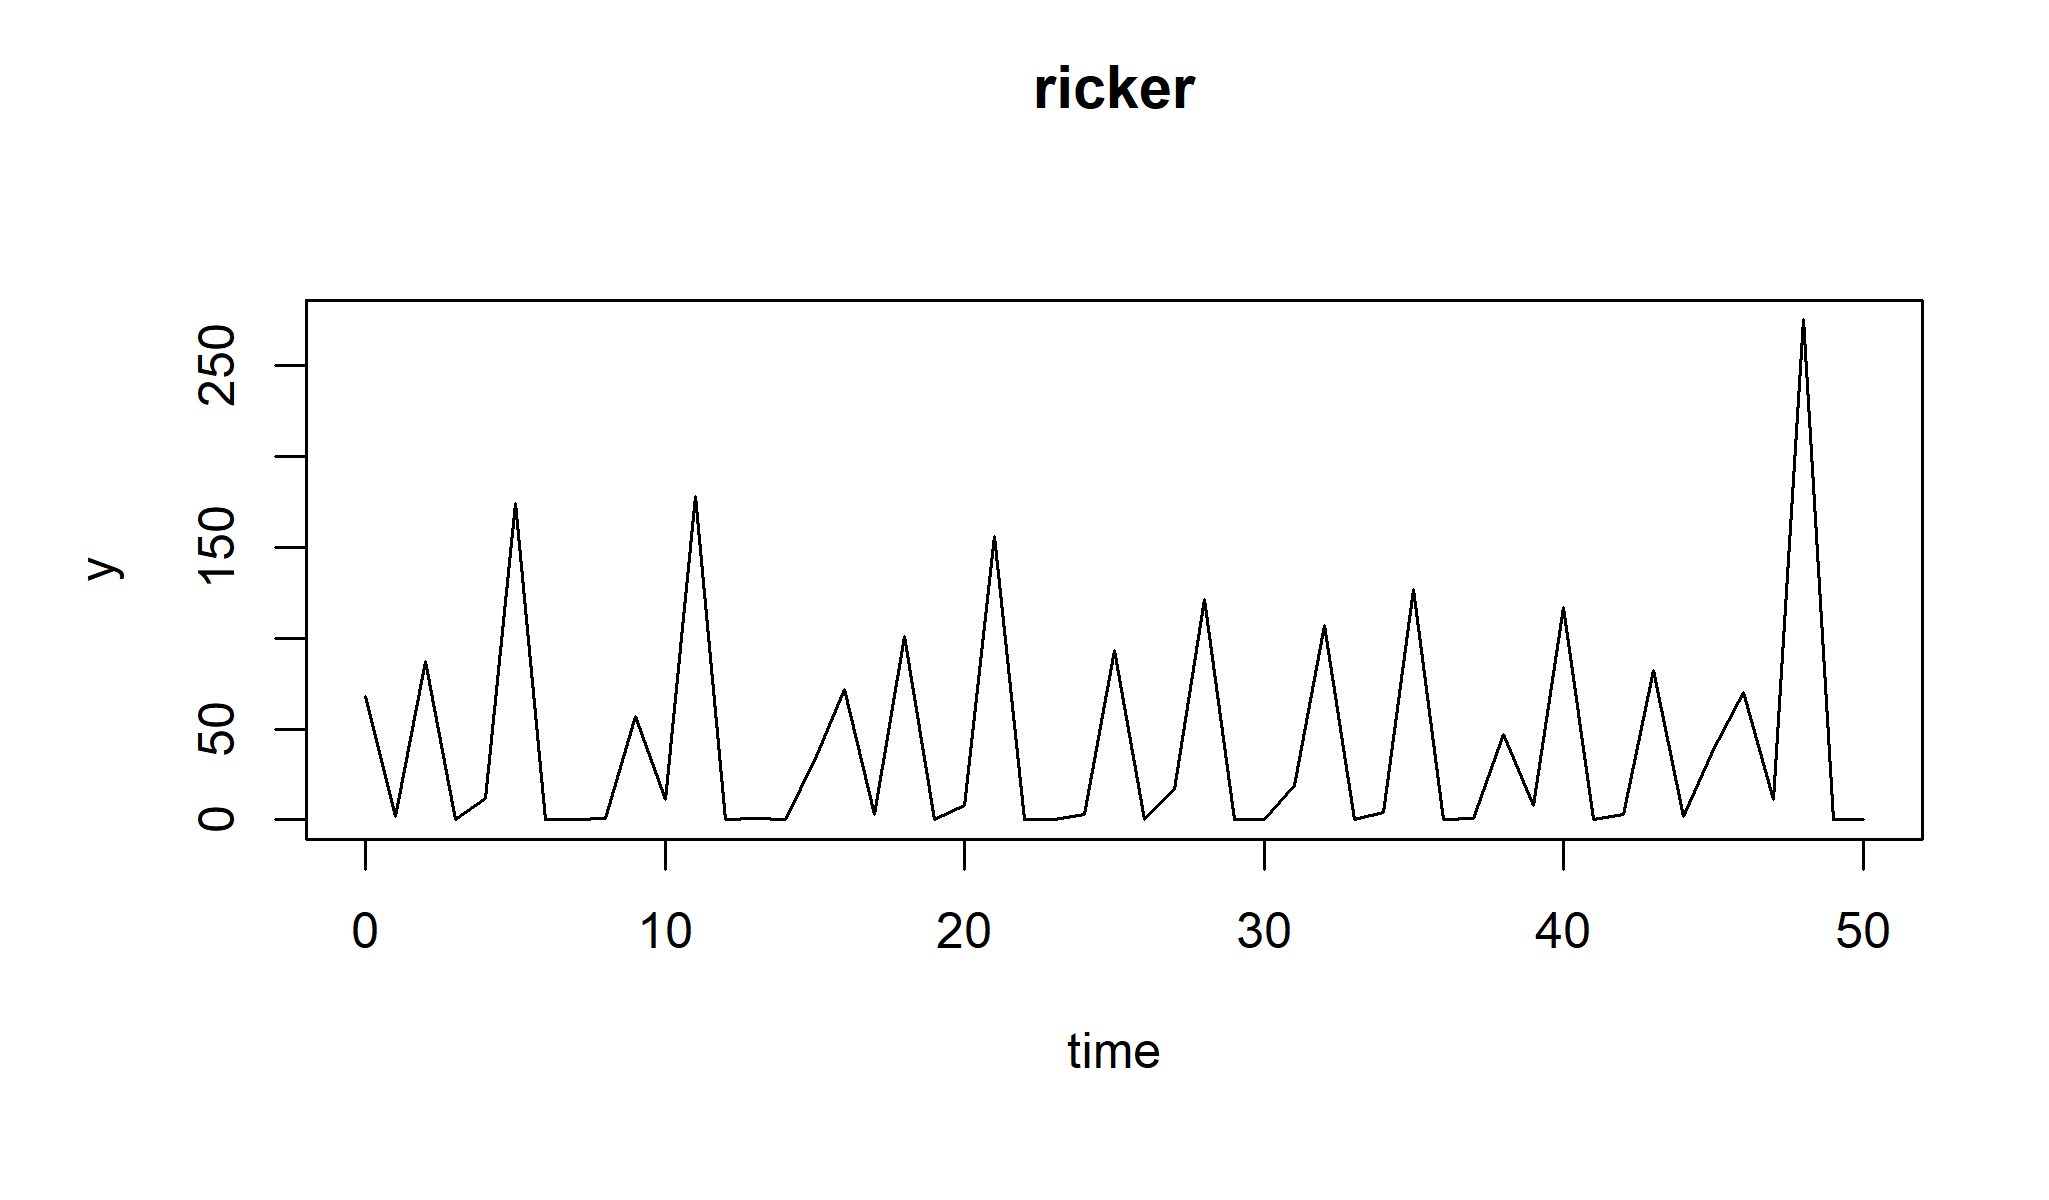
\includegraphics{figure/intro-plot-ricker-1} \end{center}

\begin{itemize}
\item
  Note that this \textbf{pomp} representation uses \texttt{N} for our
  variable \texttt{P\_n}
\item
  We can simulate by doing
\end{itemize}

\begin{Shaded}
\begin{Highlighting}[]
\NormalTok{x <-}\StringTok{ }\KeywordTok{simulate}\NormalTok{(ricker)}
\end{Highlighting}
\end{Shaded}

\begin{itemize}
\tightlist
\item
  What kind of object have we created?
\end{itemize}

\begin{Shaded}
\begin{Highlighting}[]
\KeywordTok{class}\NormalTok{(x)}
\end{Highlighting}
\end{Shaded}

\begin{verbatim}
## [1] "pomp"
## attr(,"package")
## [1] "pomp"
\end{verbatim}

\begin{Shaded}
\begin{Highlighting}[]
\KeywordTok{plot}\NormalTok{(x)}
\end{Highlighting}
\end{Shaded}

\todo[inline]{We can use two different POMP models: (1) $X_n=P_n$ and $Y_n=Y_n$ or (2) $X_n=(P_n,\log(\epsilon_n))$ and $Y_n=Y_n$. Thus, we actually chose the higher dimensional model representation. This is so that we can save the simulated draws of $\log(\epsilon_n)$ (to run diagnostics, etc).}

\begin{center}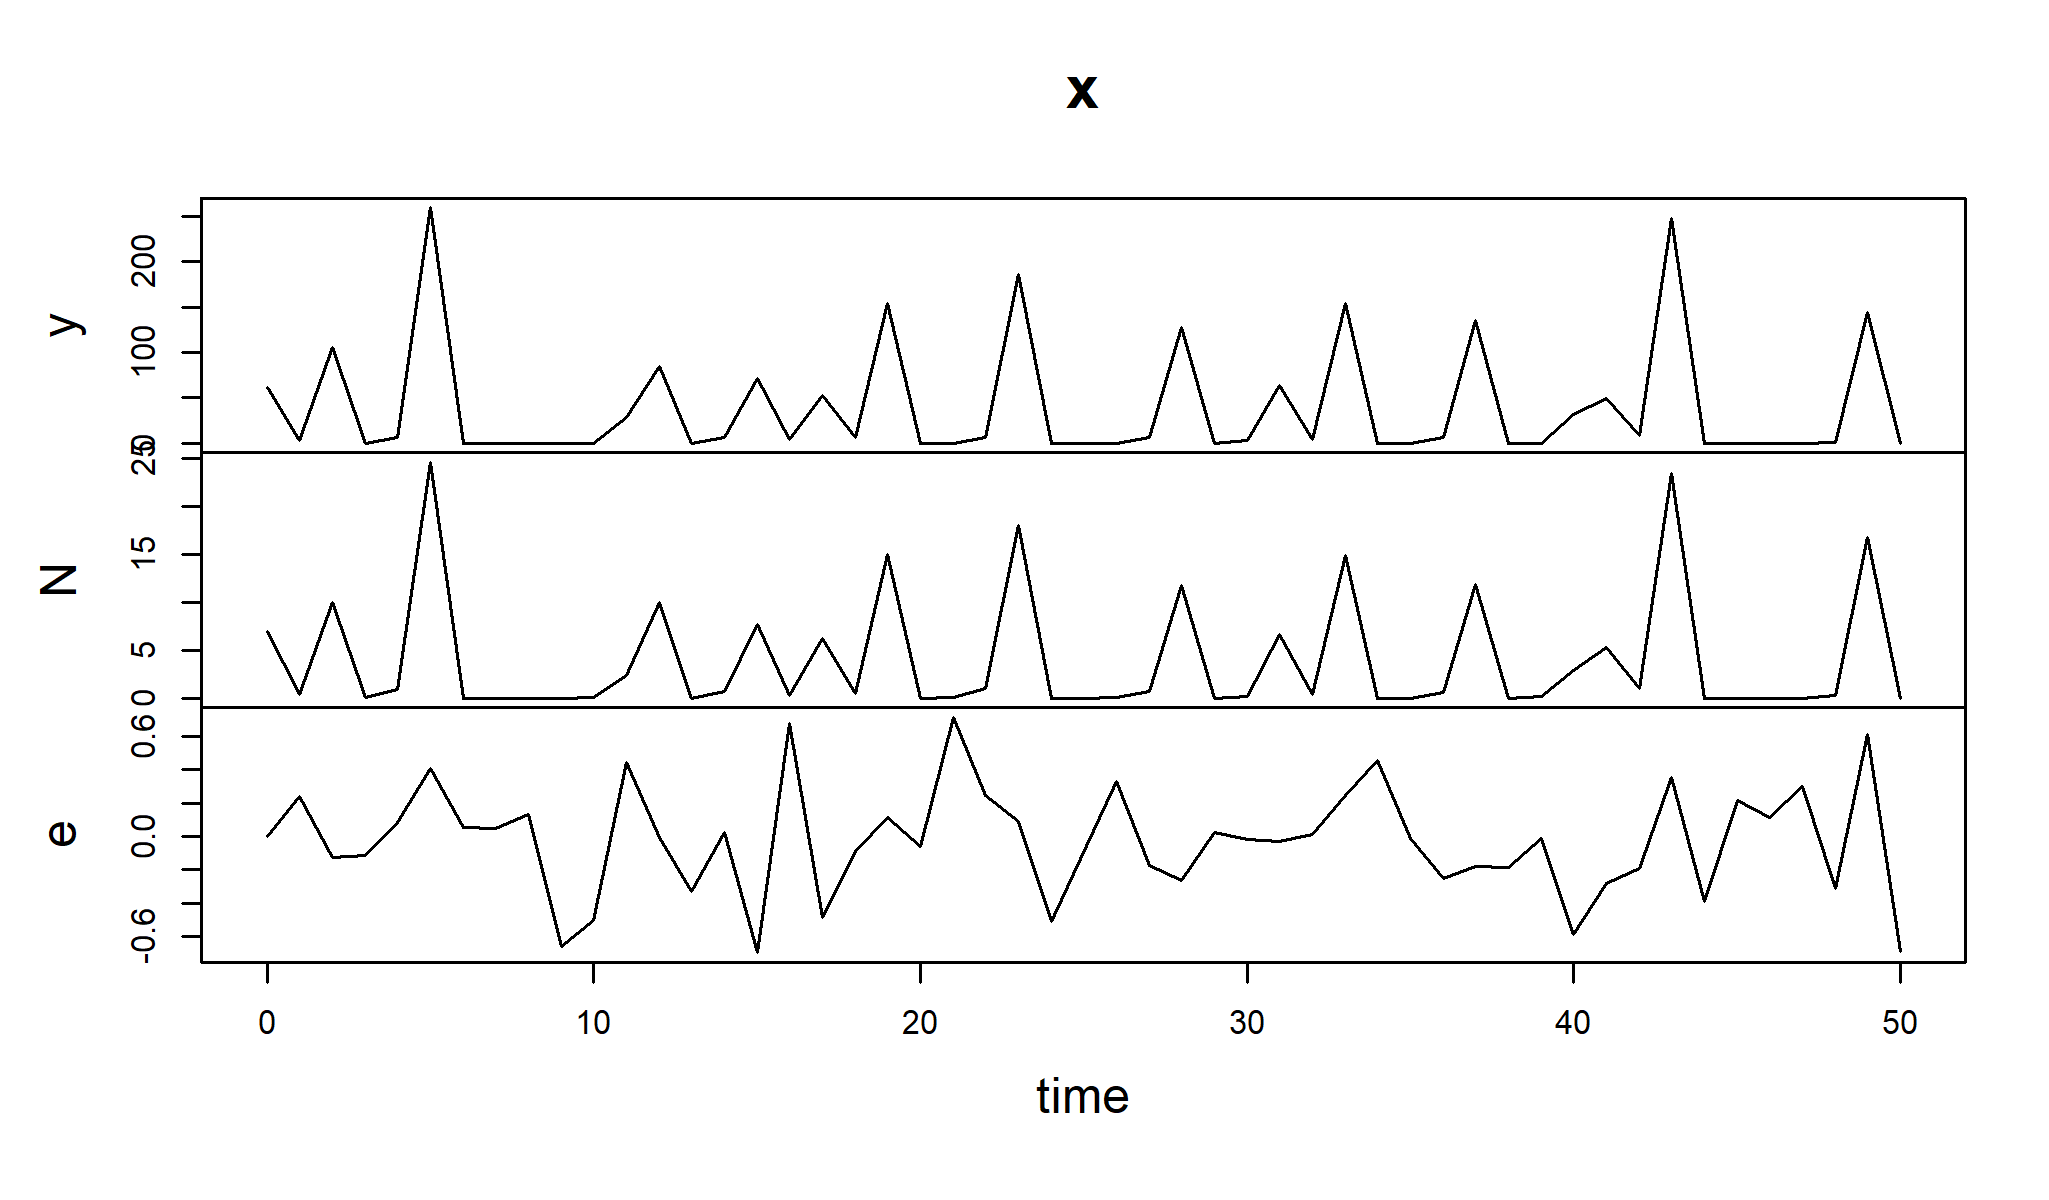
\includegraphics{figure/intro-unnamed-chunk-1-1} \end{center}

\begin{center}\rule{0.5\linewidth}{\linethickness}\end{center}

\begin{center}\rule{0.5\linewidth}{\linethickness}\end{center}

\subsubsection{Question: What is a generic
function?}\label{question-what-is-a-generic-function}

\begin{itemize}
\item
  How does the concept of a
  \href{https://en.wikipedia.org/wiki/Generic_function}{\textbf{generic
  function}} fit in with the following related concepts,

  \begin{itemize}
  \item
    \href{https://en.wikipedia.org/wiki/Object-oriented_programming}{\textbf{object-oriented
    programming}}.
  \item
    assigning a
    \href{https://en.wikipedia.org/wiki/Class_\%28computer_programming\%29}{\textbf{class}}
    to an object.
  \item
    \href{https://en.wikipedia.org/wiki/Function_overloading}{\textbf{overloading}}
    of functions or operators.
  \item
    \href{https://en.wikipedia.org/wiki/Inheritance_\%28object-oriented_programming\%29}{\textbf{inheritance}}
    between classes, when one class extends another.
  \end{itemize}
\item
  How does object-oriented programming work in R? How is this similar or
  different from any other environment in which you have seen
  object-oriented programming?
\item
  For current purposes, we don't need to be experts in object-oriented
  programming in R. However, we should know of the existence of the two
  main object-oriented systems in R,

  \begin{itemize}
  \item
    \href{http://adv-r.had.co.nz/OO-essentials.html\#s3}{\textbf{S3
    classes}}
  \item
    \href{http://adv-r.had.co.nz/S4.html}{\textbf{S4 classes}}
  \end{itemize}
\item
  We should be able to recognize when code we are using employs S3 and
  S4 classes.
\item
  We should know where to turn to for help if we find ourselves needing
  to know more details about how these work.
\item
  \textbf{pomp} uses the S4 class system, so that system is of more
  immediate relevance. Many older R packages use S3 classes.
\end{itemize}

\begin{center}\rule{0.5\linewidth}{\linethickness}\end{center}

\begin{center}\rule{0.5\linewidth}{\linethickness}\end{center}

\begin{itemize}
\item
  Why do we see more time series in the simulated \texttt{pomp} object?
\item
  We can turn a \texttt{pomp} object into a data frame:
\end{itemize}

\begin{Shaded}
\begin{Highlighting}[]
\NormalTok{y <-}\StringTok{ }\KeywordTok{as.data.frame}\NormalTok{(ricker)}
\KeywordTok{head}\NormalTok{(y)}
\end{Highlighting}
\end{Shaded}

\begin{verbatim}
##   time   y
## 1    0  68
## 2    1   2
## 3    2  87
## 4    3   0
## 5    4  12
## 6    5 174
\end{verbatim}

\begin{Shaded}
\begin{Highlighting}[]
\KeywordTok{head}\NormalTok{(}\KeywordTok{simulate}\NormalTok{(ricker,}\DataTypeTok{as.data.frame=}\OtherTok{TRUE}\NormalTok{))}
\end{Highlighting}
\end{Shaded}

\begin{verbatim}
##   time  y          N            e sim
## 1    0 68 7.00000000  0.000000000   1
## 2    1  3 0.26614785 -0.069613447   1
## 3    2 96 9.10502650 -0.001322229   1
## 4    3  0 0.06857102  0.416314640   1
## 5    4 22 3.20815215  0.114151375   1
## 6    5 86 8.95670223  0.434859137   1
\end{verbatim}

\begin{itemize}
\tightlist
\item
  We can also run multiple simulations simultaneously:
\end{itemize}

\begin{Shaded}
\begin{Highlighting}[]
\NormalTok{x <-}\StringTok{ }\KeywordTok{simulate}\NormalTok{(ricker,}\DataTypeTok{nsim=}\DecValTok{10}\NormalTok{)}
\KeywordTok{class}\NormalTok{(x)}
\end{Highlighting}
\end{Shaded}

\begin{verbatim}
## [1] "list"
\end{verbatim}

\begin{Shaded}
\begin{Highlighting}[]
\KeywordTok{sapply}\NormalTok{(x,class)}
\end{Highlighting}
\end{Shaded}

\begin{verbatim}
##  [1] "pomp" "pomp" "pomp" "pomp" "pomp" "pomp" "pomp" "pomp" "pomp" "pomp"
\end{verbatim}

\begin{Shaded}
\begin{Highlighting}[]
\NormalTok{x <-}\StringTok{ }\KeywordTok{simulate}\NormalTok{(ricker,}\DataTypeTok{nsim=}\DecValTok{10}\NormalTok{,}\DataTypeTok{as.data.frame=}\OtherTok{TRUE}\NormalTok{)}
\KeywordTok{head}\NormalTok{(x)}
\end{Highlighting}
\end{Shaded}

\begin{verbatim}
##   time   y            N          e sim
## 1    0  61 7.000000e+00  0.0000000   1
## 2    1   3 2.400265e-01 -0.1729162   1
## 3    2  53 5.293097e+00 -0.4665640   1
## 4    3  17 1.443727e+00  0.1939209   1
## 5    4 155 1.868361e+01  0.2041458   1
## 6    5   0 8.847808e-06  0.3206253   1
\end{verbatim}

\begin{Shaded}
\begin{Highlighting}[]
\KeywordTok{str}\NormalTok{(x)}
\end{Highlighting}
\end{Shaded}

\begin{verbatim}
## 'data.frame':    510 obs. of  5 variables:
##  $ time: num  0 1 2 3 4 5 6 7 8 9 ...
##  $ y   : num  61 3 53 17 155 0 0 0 13 95 ...
##  $ N   : num  7 0.24 5.29 1.44 18.68 ...
##  $ e   : num  0 -0.173 -0.467 0.194 0.204 ...
##  $ sim : Ord.factor w/ 10 levels "1"<"2"<"3"<"4"<..: 1 1 1 1 1 1 1 1 1 1 ...
\end{verbatim}

\todo[inline]{In above df, gives you observation process and state (latent) process. In pomp terminolog, N is the latent process, Y is the observed process}

Also,

\begin{Shaded}
\begin{Highlighting}[]
\NormalTok{x <-}\StringTok{ }\KeywordTok{simulate}\NormalTok{(ricker,}\DataTypeTok{nsim=}\DecValTok{9}\NormalTok{,}\DataTypeTok{as.data.frame=}\OtherTok{TRUE}\NormalTok{,}\DataTypeTok{include.data=}\OtherTok{TRUE}\NormalTok{)}
\KeywordTok{ggplot}\NormalTok{(}\DataTypeTok{data=}\NormalTok{x,}\KeywordTok{aes}\NormalTok{(}\DataTypeTok{x=}\NormalTok{time,}\DataTypeTok{y=}\NormalTok{y,}\DataTypeTok{group=}\NormalTok{sim,}\DataTypeTok{color=}\NormalTok{(sim}\OperatorTok{==}\StringTok{"data"}\NormalTok{)))}\OperatorTok{+}
\StringTok{  }\KeywordTok{geom_line}\NormalTok{()}\OperatorTok{+}\KeywordTok{guides}\NormalTok{(}\DataTypeTok{color=}\OtherTok{FALSE}\NormalTok{)}\OperatorTok{+}
\StringTok{  }\KeywordTok{facet_wrap}\NormalTok{(}\OperatorTok{~}\NormalTok{sim,}\DataTypeTok{ncol=}\DecValTok{2}\NormalTok{)}
\end{Highlighting}
\end{Shaded}

\begin{center}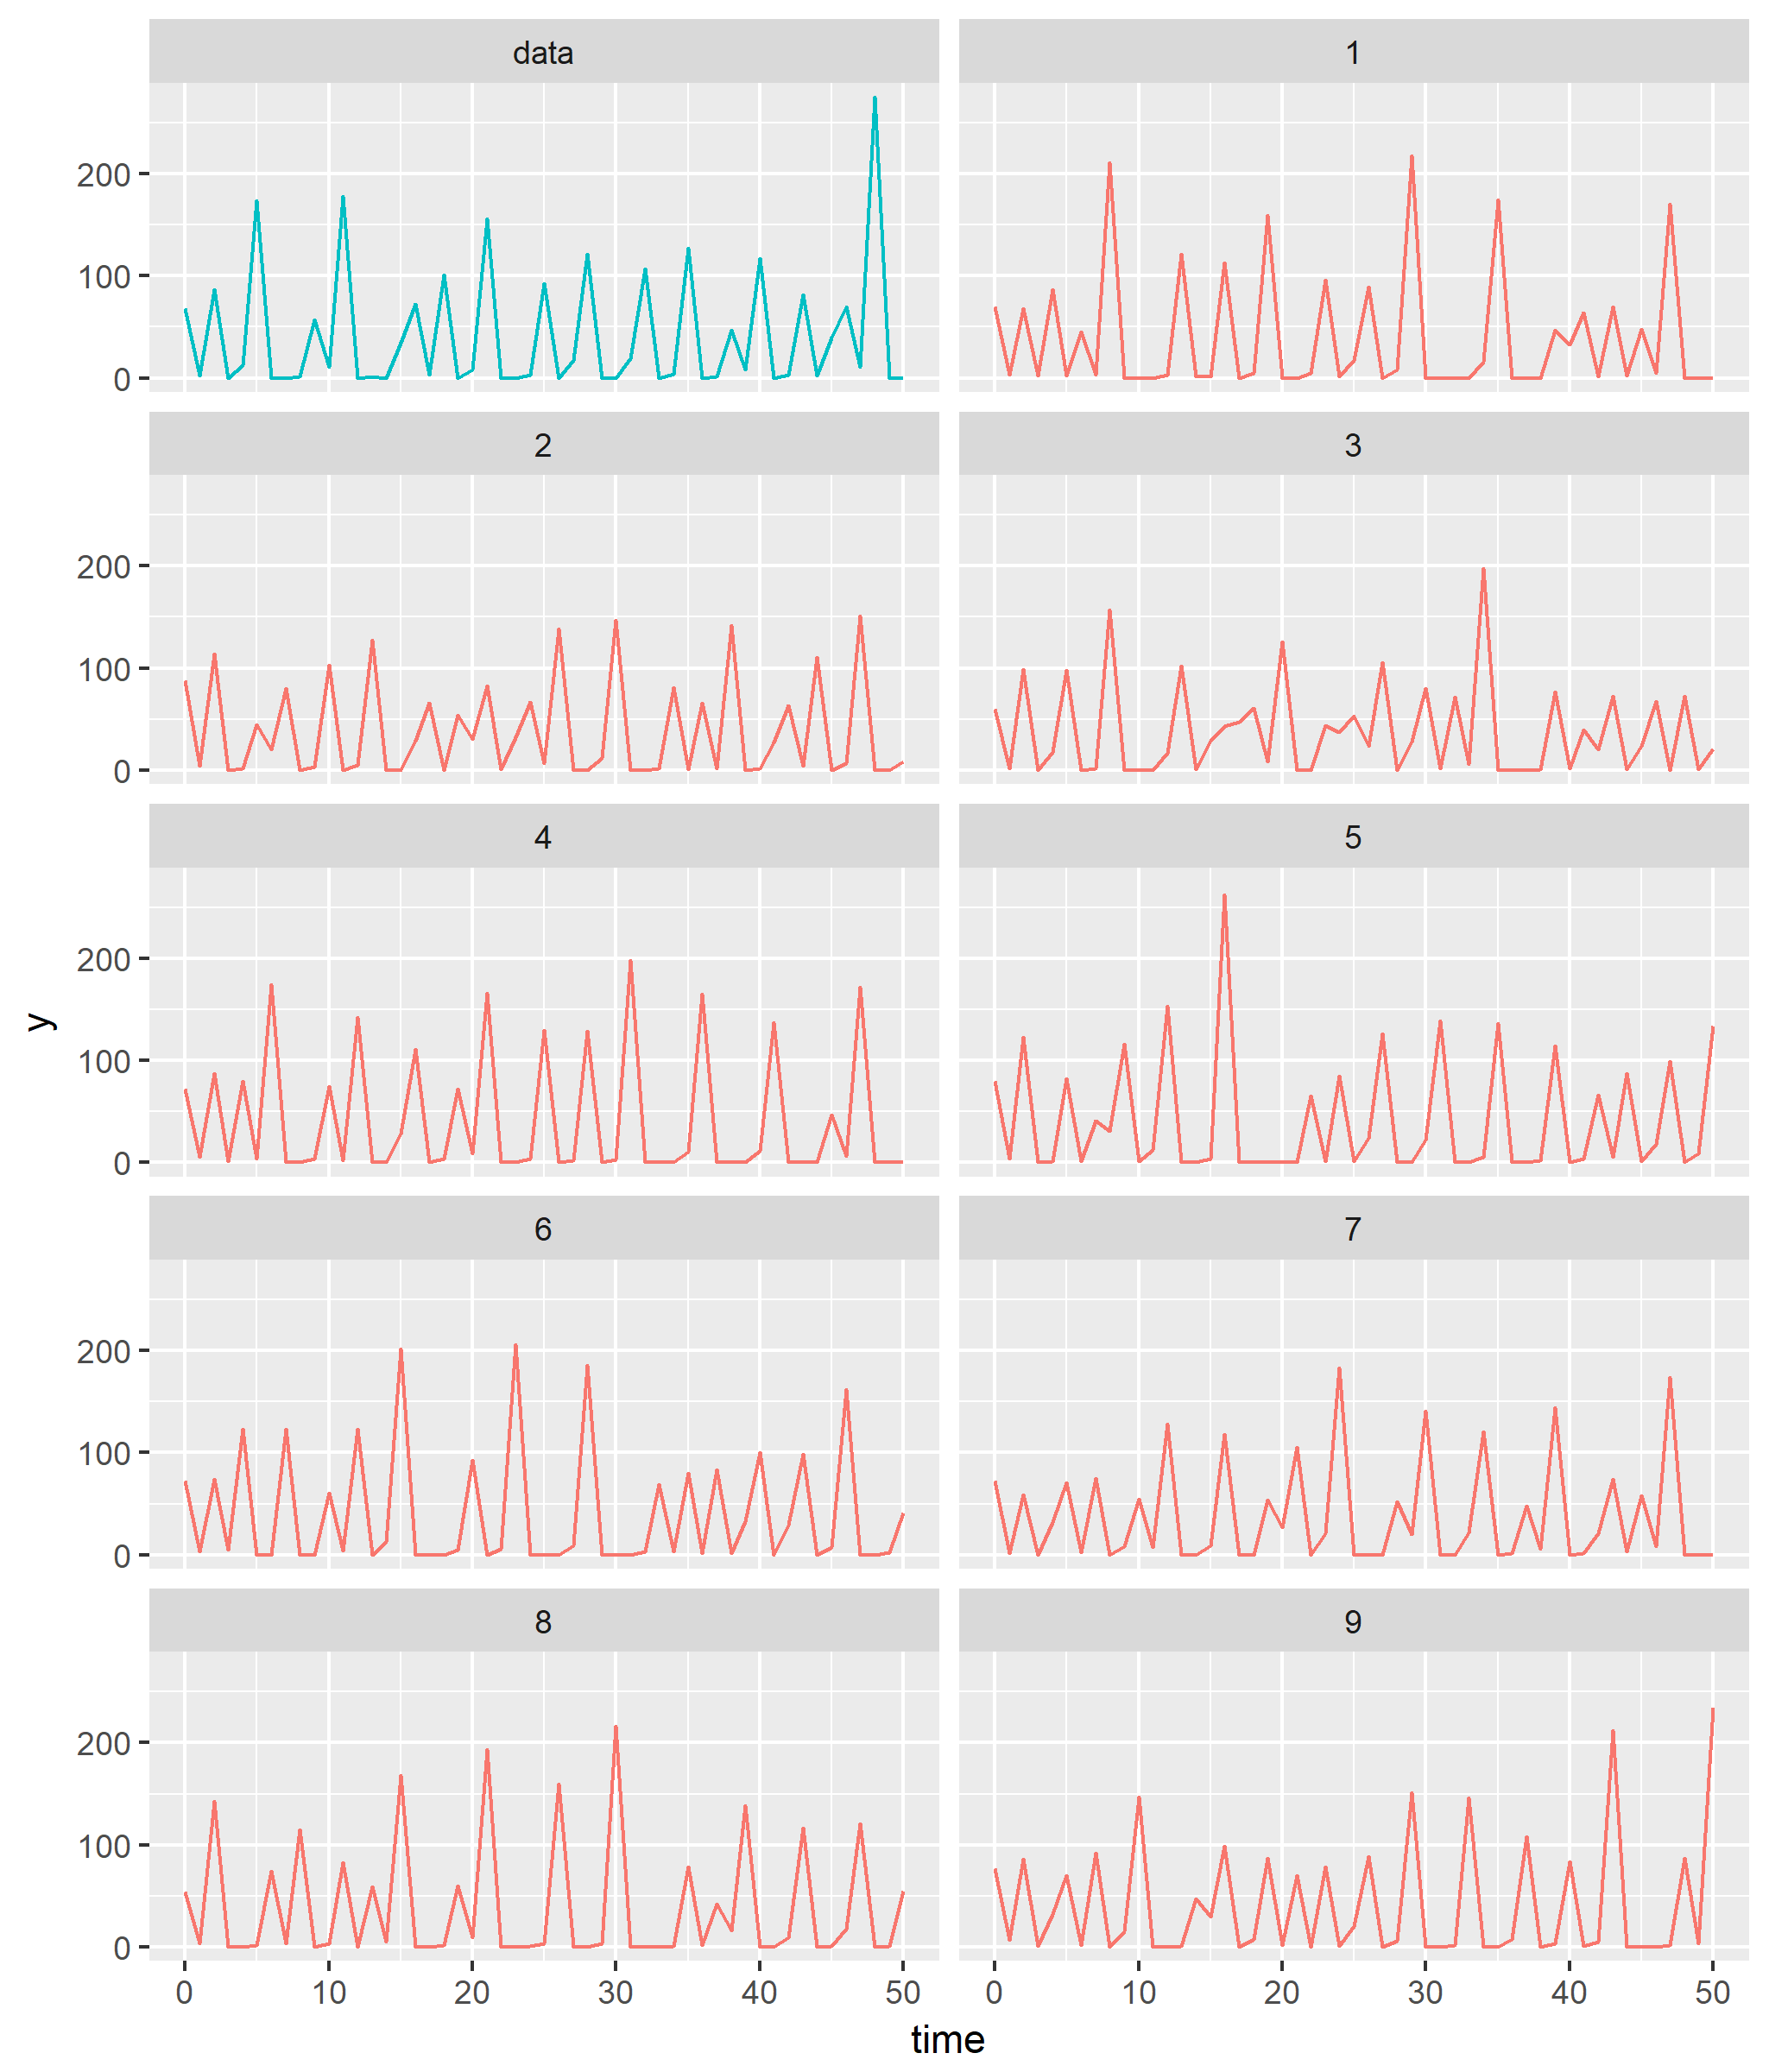
\includegraphics{figure/intro-unnamed-chunk-4-1} \end{center}

\begin{itemize}
\tightlist
\item
  We can compute a trajectory of the deterministic skeleton
\end{itemize}

\begin{Shaded}
\begin{Highlighting}[]
\NormalTok{y <-}\StringTok{ }\KeywordTok{trajectory}\NormalTok{(ricker)}
\KeywordTok{dim}\NormalTok{(y)}
\end{Highlighting}
\end{Shaded}

\begin{verbatim}
## [1]  2  1 51
\end{verbatim}

\begin{Shaded}
\begin{Highlighting}[]
\KeywordTok{dimnames}\NormalTok{(y)}
\end{Highlighting}
\end{Shaded}

\begin{verbatim}
## $variable
## [1] "N" "e"
## 
## $rep
## NULL
## 
## $time
## NULL
\end{verbatim}

\begin{Shaded}
\begin{Highlighting}[]
\KeywordTok{plot}\NormalTok{(}\KeywordTok{time}\NormalTok{(ricker),y[}\StringTok{"N"}\NormalTok{,}\DecValTok{1}\NormalTok{,],}\DataTypeTok{type=}\StringTok{"l"}\NormalTok{)}
\end{Highlighting}
\end{Shaded}

\begin{center}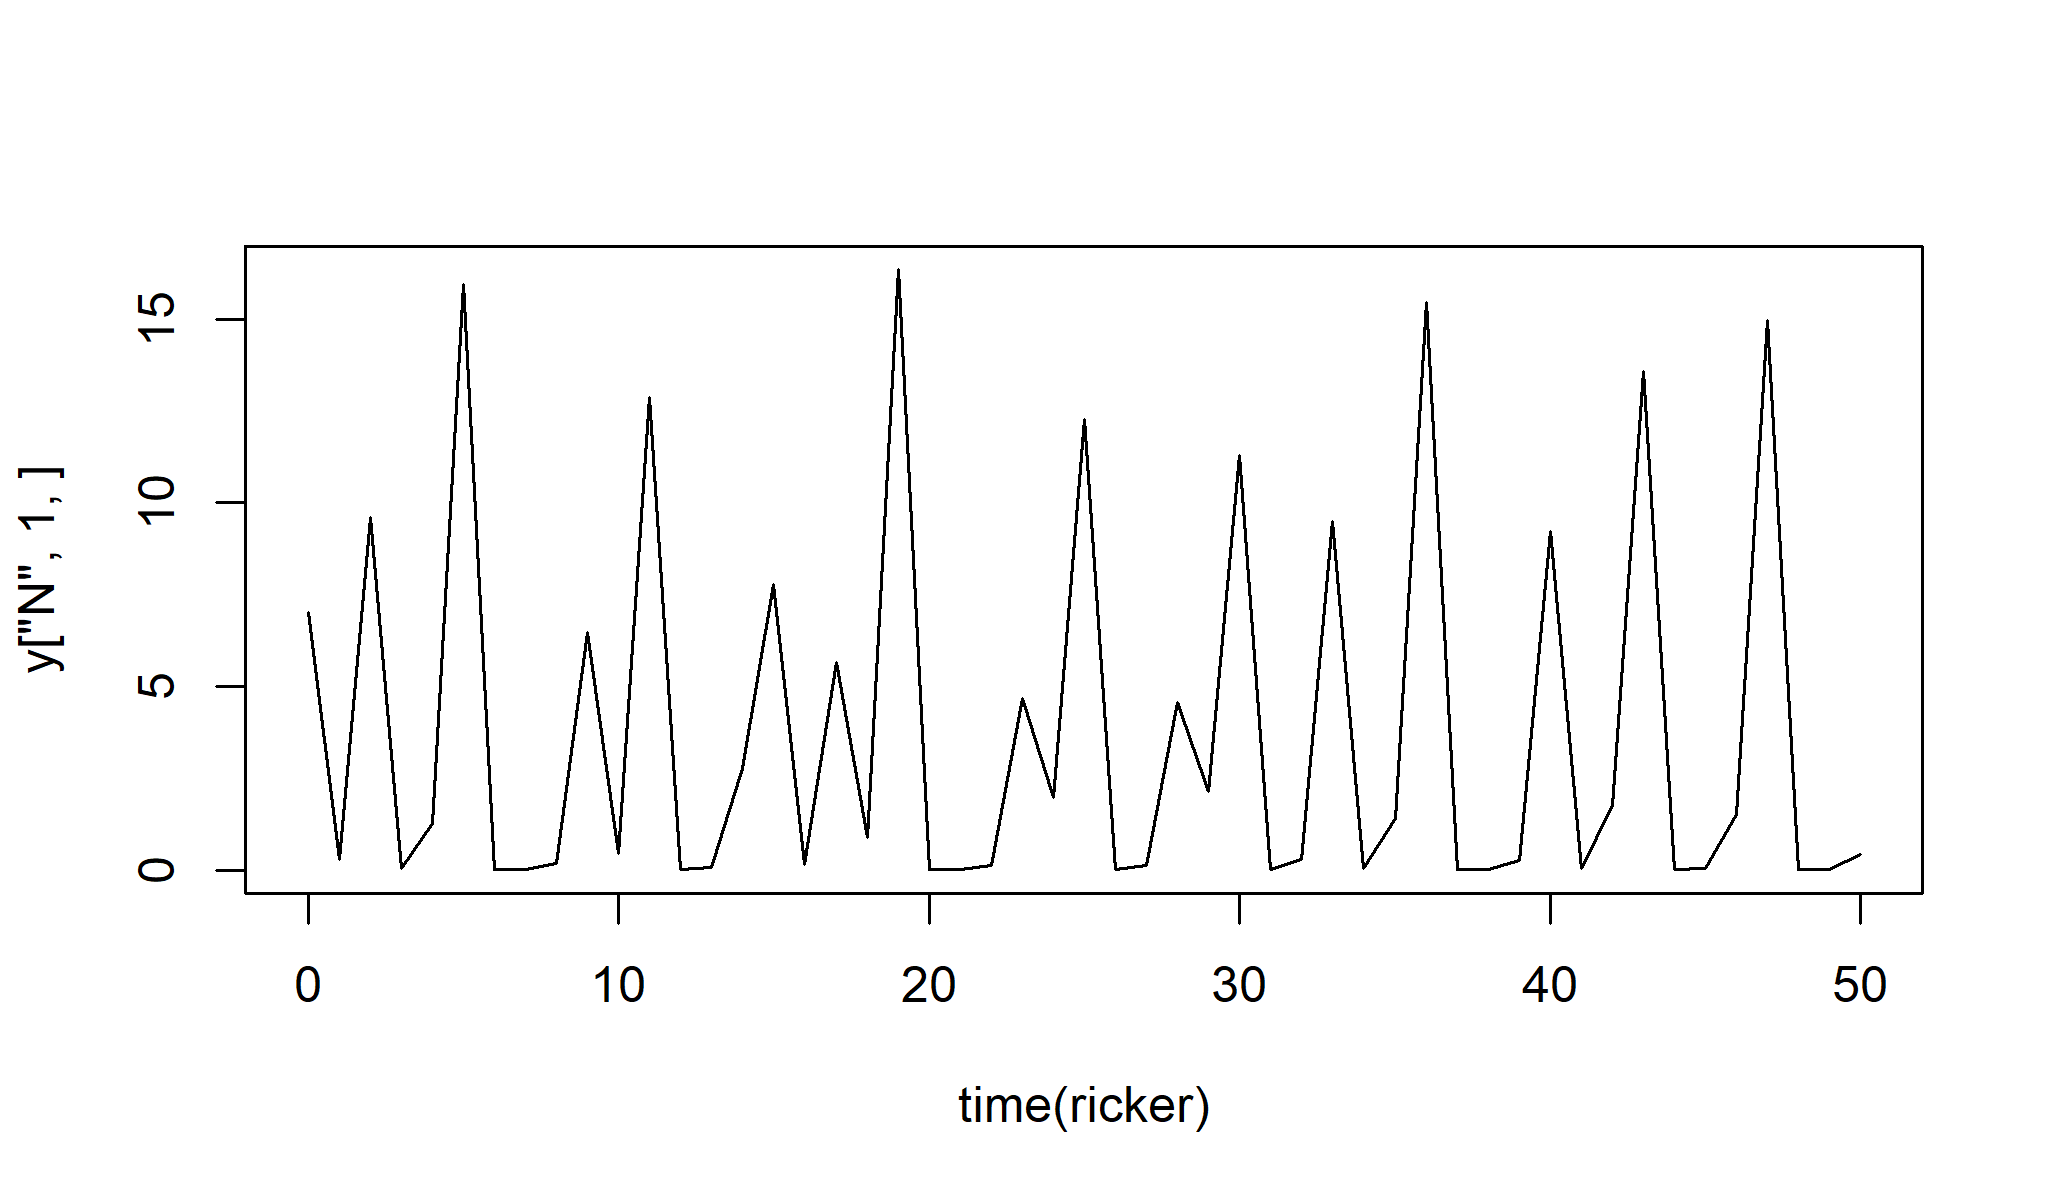
\includegraphics{figure/intro-traj-ricker-1} \end{center}

\begin{itemize}
\tightlist
\item
  Notice that \texttt{ricker} has parameters associated with it:
\end{itemize}

\begin{Shaded}
\begin{Highlighting}[]
\KeywordTok{coef}\NormalTok{(ricker)}
\end{Highlighting}
\end{Shaded}

\begin{verbatim}
##        r    sigma      phi        c      N.0      e.0 
## 44.70118  0.30000 10.00000  1.00000  7.00000  0.00000
\end{verbatim}

\todo[inline]{In output above, N.0 is the initial value of the state (latent) process}

\begin{itemize}
\item
  These are the parameters at which the simulations and deterministic
  trajectory computations above were done.
\item
  We can run these at different parameters:
\end{itemize}

\begin{Shaded}
\begin{Highlighting}[]
\NormalTok{theta <-}\StringTok{ }\KeywordTok{coef}\NormalTok{(ricker)}
\NormalTok{theta[}\KeywordTok{c}\NormalTok{(}\StringTok{"r"}\NormalTok{,}\StringTok{"N.0"}\NormalTok{)] <-}\StringTok{ }\KeywordTok{c}\NormalTok{(}\DecValTok{5}\NormalTok{,}\DecValTok{3}\NormalTok{)}
\NormalTok{y <-}\StringTok{ }\KeywordTok{trajectory}\NormalTok{(ricker,}\DataTypeTok{params=}\NormalTok{theta)}
\KeywordTok{plot}\NormalTok{(}\KeywordTok{time}\NormalTok{(ricker),y[}\StringTok{"N"}\NormalTok{,}\DecValTok{1}\NormalTok{,],}\DataTypeTok{type=}\StringTok{"l"}\NormalTok{)}
\end{Highlighting}
\end{Shaded}

\begin{center}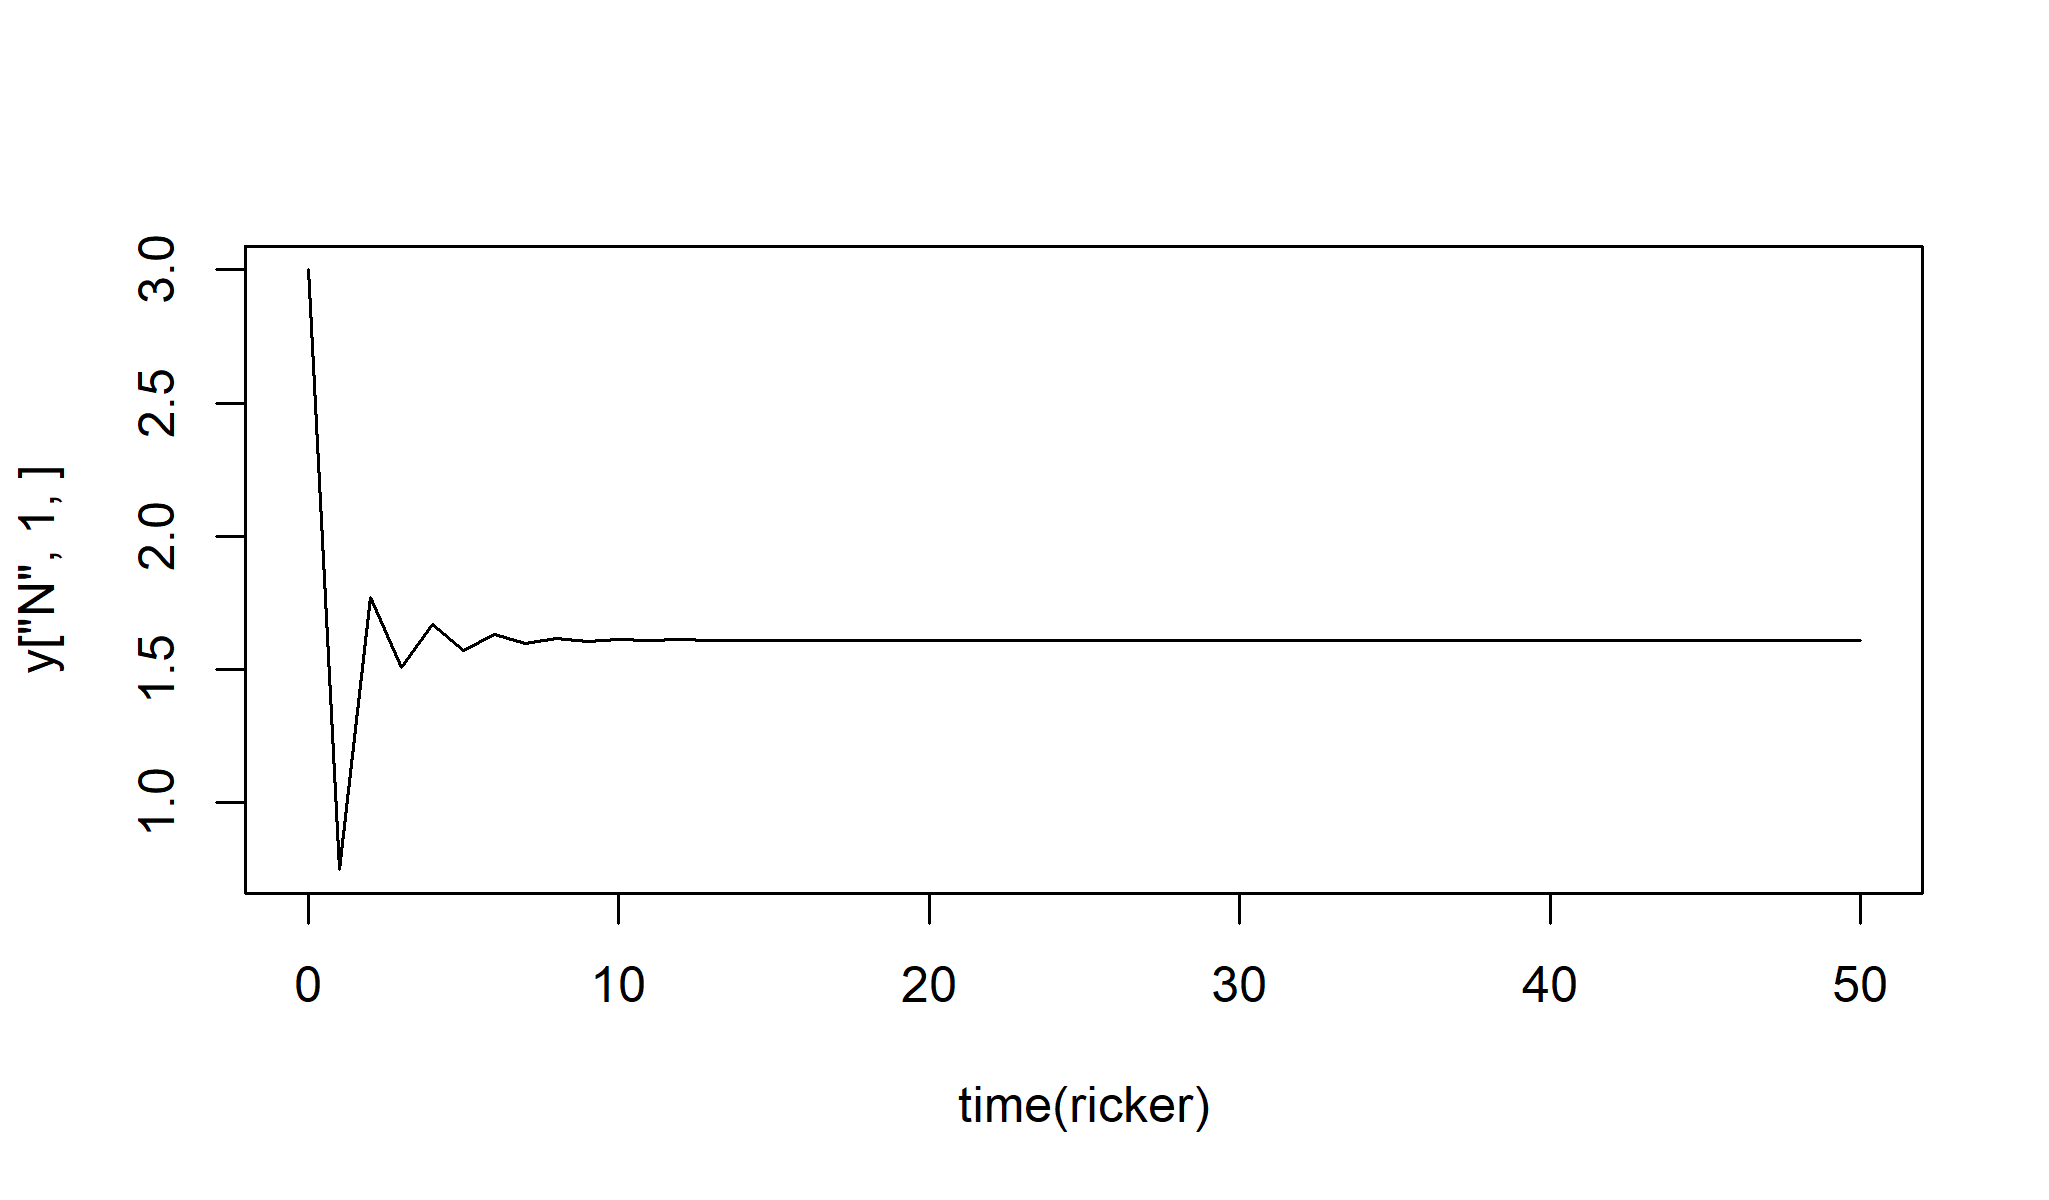
\includegraphics{figure/intro-unnamed-chunk-5-1} \end{center}
\todo[inline]{New set of parameters creates state process that converges to an equilibrium population density.}
\begin{Shaded}
\begin{Highlighting}[]
\NormalTok{x <-}\StringTok{ }\KeywordTok{simulate}\NormalTok{(ricker,}\DataTypeTok{params=}\NormalTok{theta)}
\KeywordTok{plot}\NormalTok{(x,}\DataTypeTok{var=}\StringTok{"y"}\NormalTok{)}
\end{Highlighting}
\end{Shaded}

\begin{center}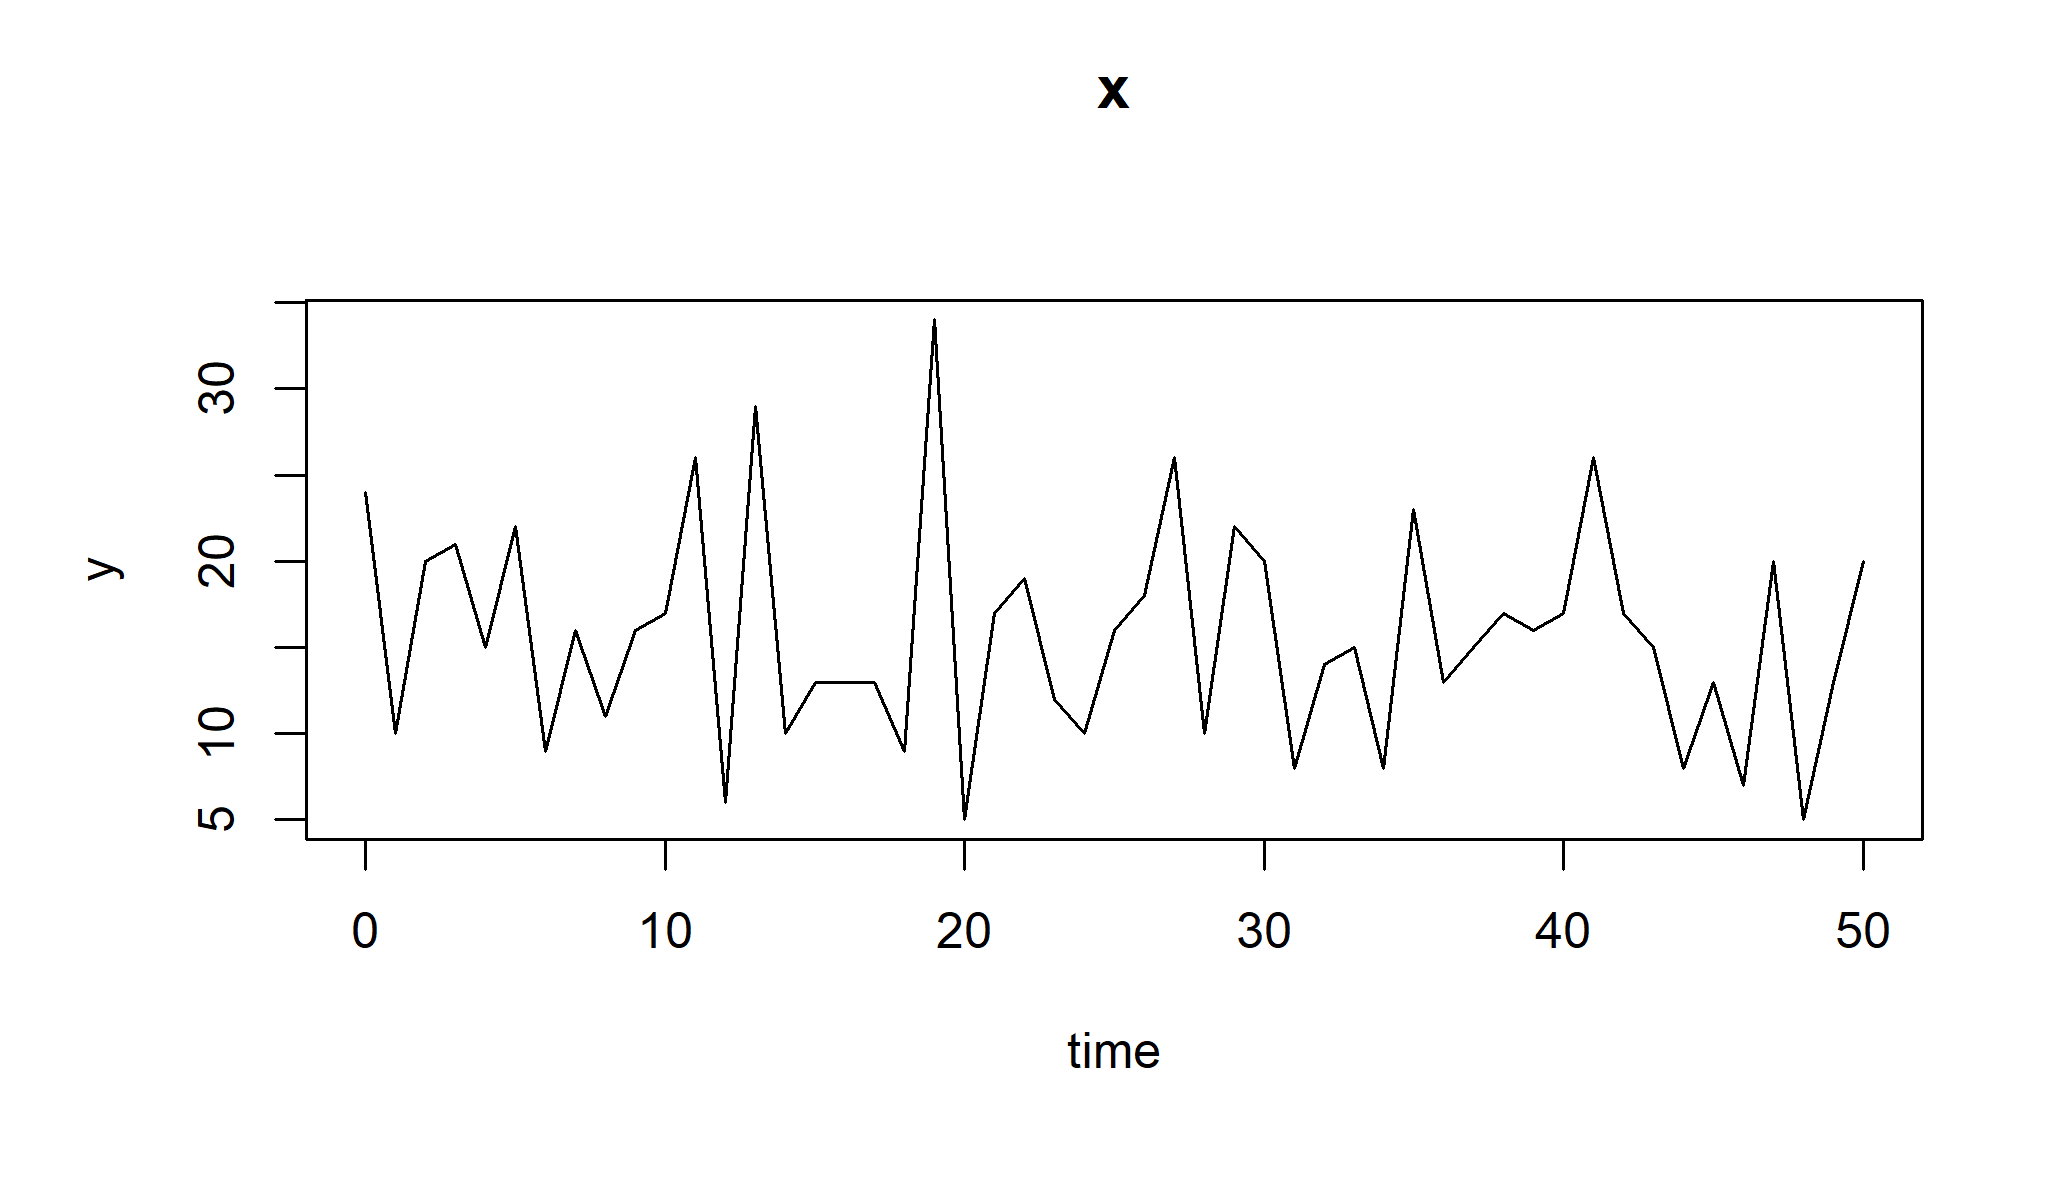
\includegraphics{figure/intro-unnamed-chunk-5-2} \end{center}

\todo[inline]{Here, the dynamics are pushing this to a stable process.}

\todo[inline]{Adding noise to a stable process doesn't have long-term effects (as in above). However, for the many gg-plots above, we have unstable processes.}

\todo[inline]{Note that in dynamics we have (1) chaotic cycles (i.e. unstable) and (2) stable cycles. In (1), a small difference in initial conditions leads to larger differences later. Here, sample paths are divergent, viewed as a function of initial conditions. In (2), there exists an equilibrium or stable limit cycle.}

\begin{itemize}
\tightlist
\item
  We can also change the parameters stored inside of \texttt{ricker}:
\end{itemize}

\begin{Shaded}
\begin{Highlighting}[]
\KeywordTok{coef}\NormalTok{(ricker,}\KeywordTok{c}\NormalTok{(}\StringTok{"r"}\NormalTok{,}\StringTok{"N.0"}\NormalTok{,}\StringTok{"sigma"}\NormalTok{)) <-}\StringTok{ }\KeywordTok{c}\NormalTok{(}\DecValTok{39}\NormalTok{,}\FloatTok{0.5}\NormalTok{,}\DecValTok{1}\NormalTok{)}
\KeywordTok{coef}\NormalTok{(ricker)}
\end{Highlighting}
\end{Shaded}

\begin{verbatim}
##     r sigma   phi     c   N.0   e.0 
##  39.0   1.0  10.0   1.0   0.5   0.0
\end{verbatim}

\todo[inline]{The c parameter above is in front of $-P_n$ in the Ricker equation in R2. Here, it's just 1.}

\begin{Shaded}
\begin{Highlighting}[]
\KeywordTok{plot}\NormalTok{(}\KeywordTok{simulate}\NormalTok{(ricker),}\DataTypeTok{var=}\StringTok{"y"}\NormalTok{)}
\end{Highlighting}
\end{Shaded}

\begin{center}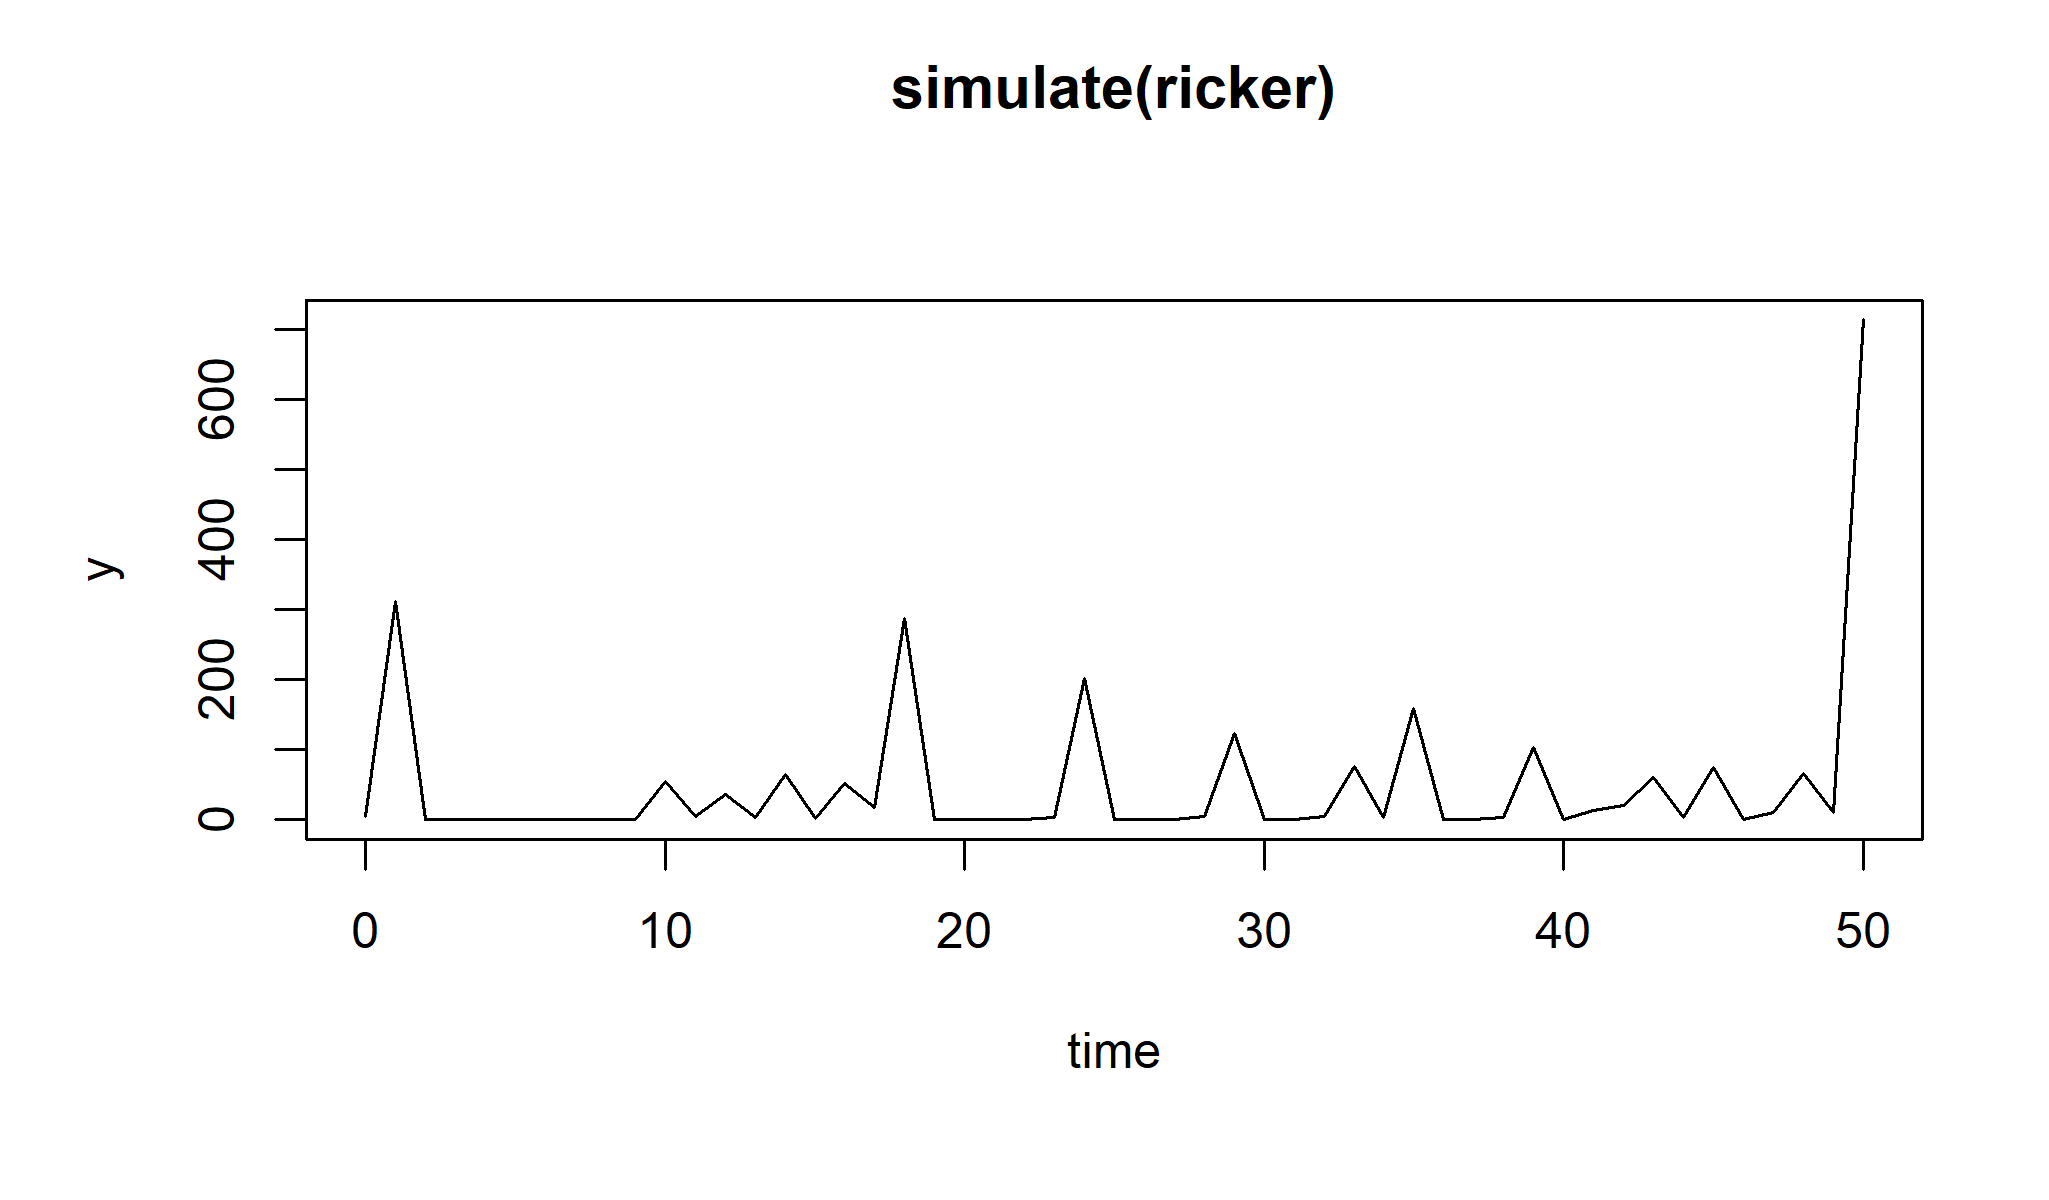
\includegraphics{figure/intro-unnamed-chunk-6-1} \end{center}

\begin{itemize}
\tightlist
\item
  In all of the above, it's possible to work with more than one set of
  parameters at a time. For example:
\end{itemize}

\begin{Shaded}
\begin{Highlighting}[]
\NormalTok{p <-}\StringTok{ }\KeywordTok{parmat}\NormalTok{(}\KeywordTok{coef}\NormalTok{(ricker),}\DecValTok{500}\NormalTok{)}
\KeywordTok{dim}\NormalTok{(p); }\KeywordTok{dimnames}\NormalTok{(p)}
\end{Highlighting}
\end{Shaded}

\begin{verbatim}
## [1]   6 500
\end{verbatim}

\begin{verbatim}
## $variable
## [1] "r"     "sigma" "phi"   "c"     "N.0"   "e.0"  
## 
## $rep
## NULL
\end{verbatim}

\begin{Shaded}
\begin{Highlighting}[]
\NormalTok{p[}\StringTok{"r"}\NormalTok{,] <-}\StringTok{ }\KeywordTok{seq}\NormalTok{(}\DataTypeTok{from=}\DecValTok{2}\NormalTok{,}\DataTypeTok{to=}\DecValTok{40}\NormalTok{,}\DataTypeTok{length=}\DecValTok{500}\NormalTok{)}
\NormalTok{y <-}\StringTok{ }\KeywordTok{trajectory}\NormalTok{(ricker,}\DataTypeTok{params=}\NormalTok{p,}\DataTypeTok{times=}\DecValTok{200}\OperatorTok{:}\DecValTok{1000}\NormalTok{)}
\KeywordTok{matplot}\NormalTok{(p[}\StringTok{"r"}\NormalTok{,],y[}\StringTok{"N"}\NormalTok{,,],}\DataTypeTok{pch=}\StringTok{"."}\NormalTok{,}\DataTypeTok{col=}\StringTok{'black'}\NormalTok{,}\DataTypeTok{xlab=}\StringTok{'r'}\NormalTok{,}\DataTypeTok{ylab=}\StringTok{'N'}\NormalTok{,}\DataTypeTok{log=}\StringTok{'x'}\NormalTok{)}
\end{Highlighting}
\end{Shaded}

\begin{center}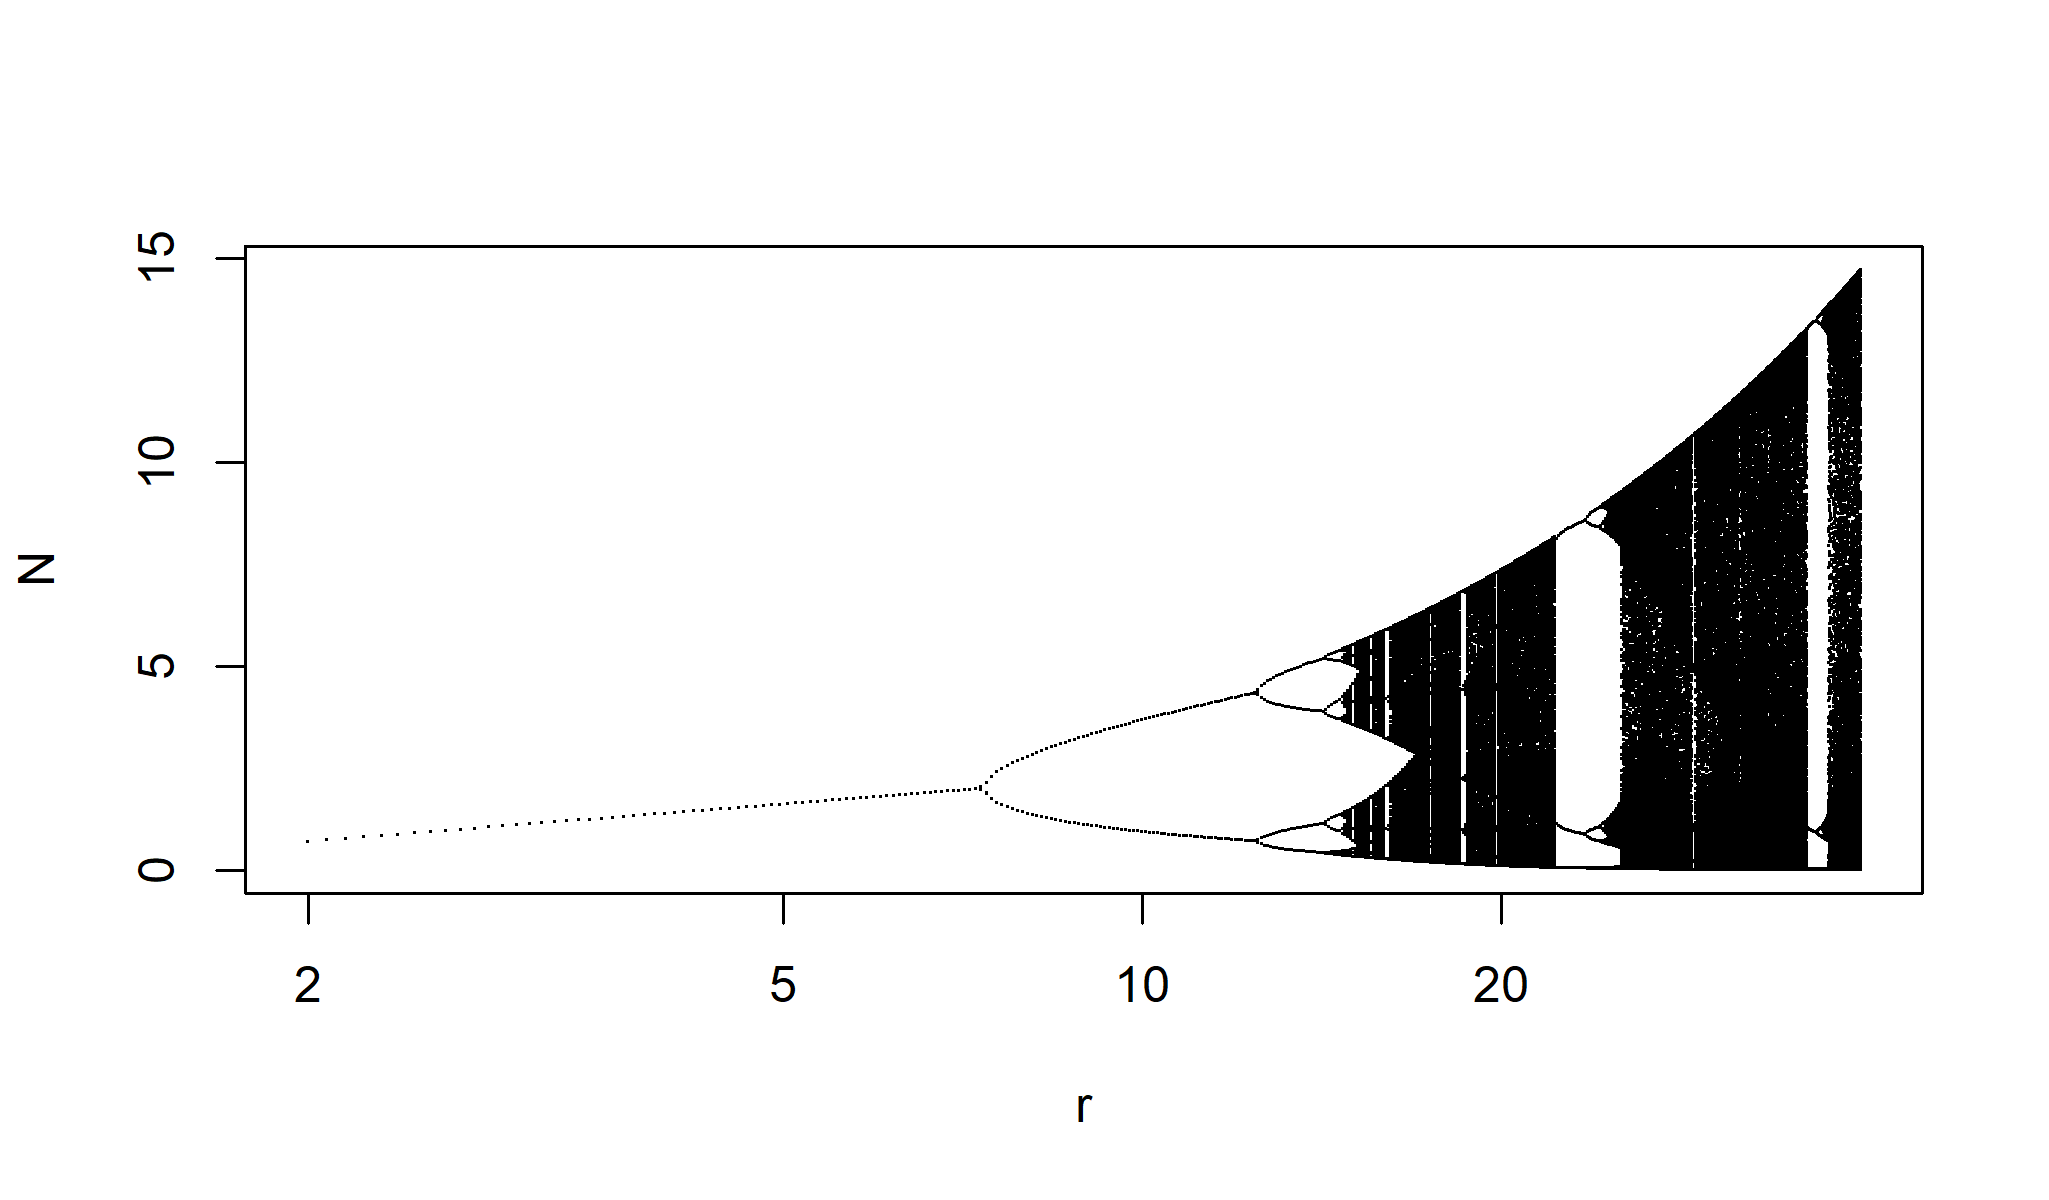
\includegraphics{figure/intro-bifdiag-1} \end{center}

\begin{itemize}
\item
  This figure is called a
  \href{https://en.wikipedia.org/wiki/Bifurcation_diagram}{bifurcation
  diagram} for the Ricker map. The Ricker map is another name for the
  Ricker equation: the Ricker equation defines a recursion, and these
  recursions are often called maps when mathematically studying their
  behavior.

  \begin{itemize}
  \item
    How do you interpret this bifurcation diagram?
  \item
    What does it mean when the single line for small values of \(r\)
    splits into a double line, around \(r=0.8\)?
  \item
    What does it mean when solid vertical lines appear, around \(r=18\)?
  \item
    A bifurcation diagram like this can only be computed for a
    deterministic map. Why? However, the bifurcation diagram for the
    deterministic skeleton can be useful to help understand a stochastic
    process. We'll see an example later in this chapter.
  \item
    Look at the R code for the bifurcation diagram. Notice that the
    first 200 iterations of the Ricker map are discarded, by setting
    \texttt{times=200:1000}. Why? This is a technique called
    \textbf{burn-in}, by analogy with an
    \href{https://en.wikipedia.org/wiki/Burn-in}{industrial technique by
    the same name}. Burn-in is a standard technique in Markov chain
    Monte Carlo, as described in the
    \href{https://en.wikipedia.org/wiki/Metropolis\%E2\%80\%93Hastings_algorithm}{Wikipedia
    article on the Metropolis-Hastings algorithm}: ``The Markov chain is
    started from an arbitrary initial value and the algorithm is run for
    many iterations until this initial state is forgotten. These
    samples, which are discarded, are known as burn-in.'' The concept of
    burn-in applies to any simulation study where one is interested in
    simulating the steady state of a dynamic system, ignoring the
    \href{https://en.wikipedia.org/wiki/Transient_response}{transient
    behavior} due to the choice of starting values for the simulation.
  \end{itemize}
\item
  More information on manipulating and extracting information from
  \texttt{pomp} objects can be viewed in the help pages
  (\texttt{methods?pomp}).
\item
  There are a number of other examples included with the package. Do
  \texttt{pompExamples()} to see a list of these.
\end{itemize}

\begin{center}\rule{0.5\linewidth}{\linethickness}\end{center}

\begin{center}\rule{0.5\linewidth}{\linethickness}\end{center}

\subsection{\texorpdfstring{Inference algorithms in
\textbf{pomp}}{Inference algorithms in pomp}}\label{inference-algorithms-in-pomp}

\begin{itemize}
\item
  \textbf{pomp} provides a wide range of inference algorithms. We'll
  learn about these in detail soon, but for now, let's just look at some
  of their general features.
\item
  The \texttt{pfilter} function runs a simple \textbf{particle filter},
  which is a Monte Carlo algorithm that can be used to evaluate the
  likelihood at a particular set of parameters. One uses the \texttt{Np}
  argument to specify the number of particles to use:
\end{itemize}

\begin{Shaded}
\begin{Highlighting}[]
\NormalTok{pf <-}\StringTok{ }\KeywordTok{pfilter}\NormalTok{(ricker,}\DataTypeTok{Np=}\DecValTok{1000}\NormalTok{)}
\KeywordTok{class}\NormalTok{(pf)}
\end{Highlighting}
\end{Shaded}

\begin{verbatim}
## [1] "pfilterd.pomp"
## attr(,"package")
## [1] "pomp"
\end{verbatim}

\begin{Shaded}
\begin{Highlighting}[]
\KeywordTok{plot}\NormalTok{(pf)}
\end{Highlighting}
\end{Shaded}

\begin{center}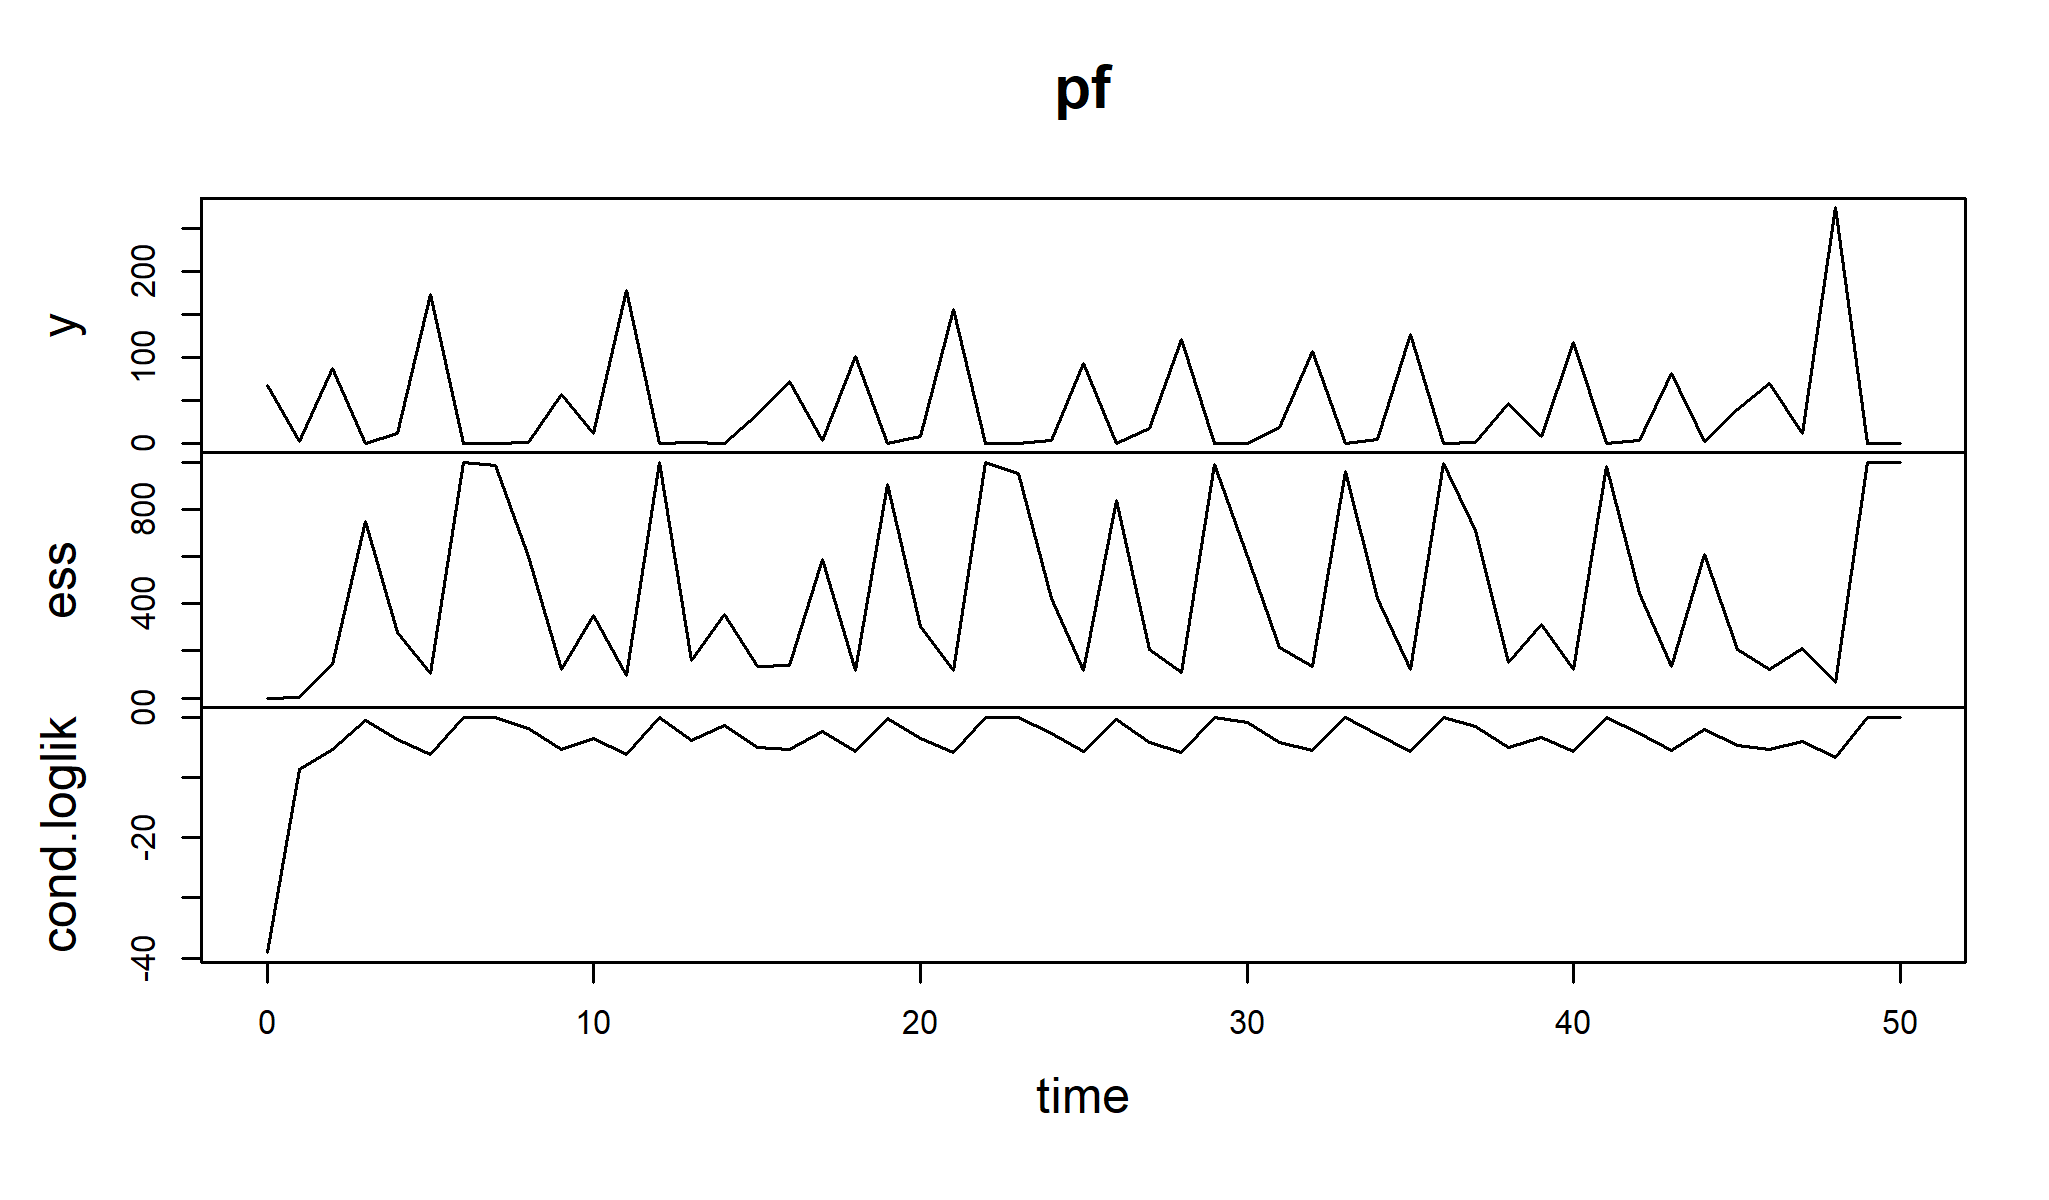
\includegraphics{figure/intro-pfilter1-1} \end{center}

\todo[inline]{ess -- effective sample size (from MCMC). The CLL is the conditional log-likelihood: $f_{Y_n|Y_{1:n-1}}$ for $n=1,\cdots, N$}

\begin{Shaded}
\begin{Highlighting}[]
\KeywordTok{logLik}\NormalTok{(pf)}
\end{Highlighting}
\end{Shaded}

\begin{verbatim}
## [1] -200.5362
\end{verbatim}

\begin{itemize}
\item
  Note that \texttt{pfilter} returns an object of class
  \texttt{pfilterd.pomp}. This is the general rule: inference algorithms
  return objects that are \texttt{pomp} objects with additional
  information. The package provides tools to extract this information.
\item
  We can run the particle filter again by doing
\end{itemize}

\begin{Shaded}
\begin{Highlighting}[]
\NormalTok{pf <-}\StringTok{ }\KeywordTok{pfilter}\NormalTok{(pf)}
\KeywordTok{logLik}\NormalTok{(pf)}
\end{Highlighting}
\end{Shaded}

\begin{verbatim}
## [1] -200.7444
\end{verbatim}

which has the result of running the same computation again.

\begin{itemize}
\item
  Note that, because the particle filter is a Monte Carlo algorithm, we
  get a slightly different estimate of the log likelihood.
\item
  Note that, by default, running \texttt{pfilter} on a
  \texttt{pfilterd.pomp} object causes the computation to be re-run with
  the same parameters as before. Any additional arguments we add
  override these defaults. This is the general rule in \textbf{pomp}.
  For example,
\end{itemize}

\begin{Shaded}
\begin{Highlighting}[]
\NormalTok{pf <-}\StringTok{ }\KeywordTok{pfilter}\NormalTok{(pf,}\DataTypeTok{Np=}\DecValTok{100}\NormalTok{)}
\KeywordTok{logLik}\NormalTok{(pf)}
\end{Highlighting}
\end{Shaded}

\begin{verbatim}
## [1] -201.9509
\end{verbatim}

Here, the particle filtering has been performed with only 100 particles.

\begin{center}\rule{0.5\linewidth}{\linethickness}\end{center}

\begin{center}\rule{0.5\linewidth}{\linethickness}\end{center}

\subsection{\texorpdfstring{Building a custom \texttt{pomp}
object}{Building a custom pomp object}}\label{building-a-custom-pomp-object}

A real \textbf{pomp} data analysis begins with constructing one or more
\texttt{pomp} objects to hold the data and the model or models under
consideration. We'll illustrate this process a dataset of the abundance
of the \href{https://en.wikipedia.org/wiki/Great_tit}{great tit
(\emph{Parus major})} in Wytham Wood, near Oxford {[}@mccleery91{]}.

Download and plot the data:

\begin{Shaded}
\begin{Highlighting}[]
\NormalTok{dat <-}\StringTok{ }\KeywordTok{read.csv}\NormalTok{(}\StringTok{"parus.csv"}\NormalTok{)}
\KeywordTok{head}\NormalTok{(dat)}
\end{Highlighting}
\end{Shaded}

\begin{verbatim}
##   year pop
## 1 1960 148
## 2 1961 258
## 3 1962 185
## 4 1963 170
## 5 1964 267
## 6 1965 239
\end{verbatim}

\begin{Shaded}
\begin{Highlighting}[]
\KeywordTok{plot}\NormalTok{(pop}\OperatorTok{~}\NormalTok{year,}\DataTypeTok{data=}\NormalTok{dat,}\DataTypeTok{type=}\StringTok{'o'}\NormalTok{)}
\end{Highlighting}
\end{Shaded}

\begin{center}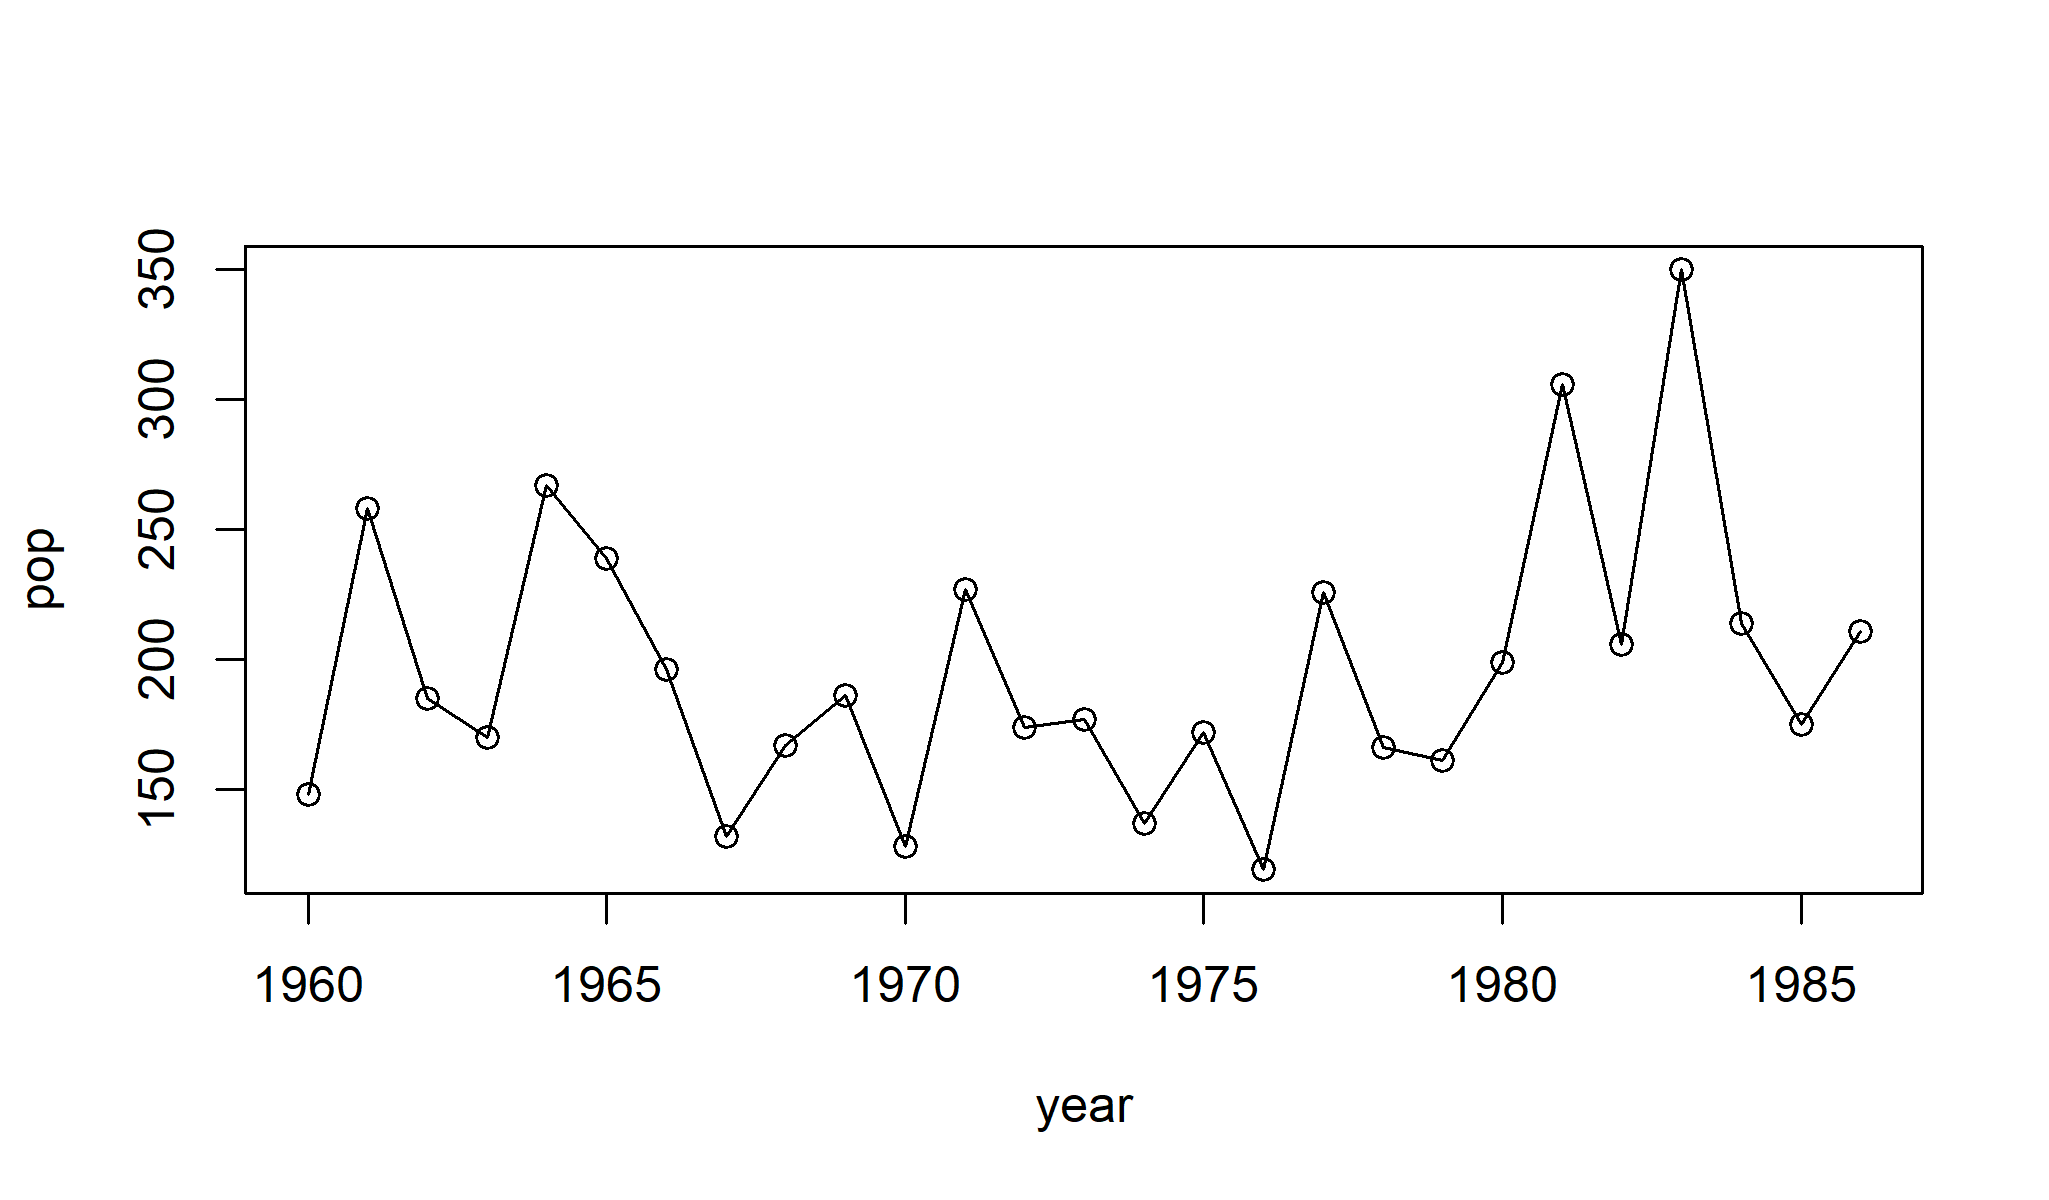
\includegraphics{figure/intro-parus-data-1} \end{center}

Let's suppose that we want to fit the stochastic Ricker model discussed
above to these data.

The call to construct a \texttt{pomp} object is, naturally enough,
\texttt{pomp}. Documentation on this function can be had by doing
\texttt{?pomp}. Do \texttt{class?pomp} to get documentation on the
\texttt{pomp} class. Learn about the various things you can do once you
have a \texttt{pomp} object by doing \texttt{methods?pomp} and following
the links therein. Read an overview of the package as a whole with links
to its main features by doing \texttt{package?pomp}. A complete index of
the functions in \textbf{pomp} is returned by the command
\texttt{library(help=pomp)}. Finally, the home page for the
\texttt{pomp} project is (\url{http://kingaa.github.io/pomp}); there you
have access to the complete source code, manuals, mailing lists, etc.

\begin{Shaded}
\begin{Highlighting}[]
\KeywordTok{require}\NormalTok{(pomp)}
\NormalTok{parus <-}\StringTok{ }\KeywordTok{pomp}\NormalTok{(dat,}\DataTypeTok{times=}\StringTok{"year"}\NormalTok{,}\DataTypeTok{t0=}\DecValTok{1959}\NormalTok{)}
\end{Highlighting}
\end{Shaded}

The \texttt{times} argument specifies that the column labelled ``year''
gives the measurement times; \texttt{t0} is the ``zero-time'', the time
at which the state process will be initialized. We've set it to one year
prior to the beginning of the data. Plot it:

\begin{Shaded}
\begin{Highlighting}[]
\KeywordTok{plot}\NormalTok{(parus)}
\end{Highlighting}
\end{Shaded}

\begin{center}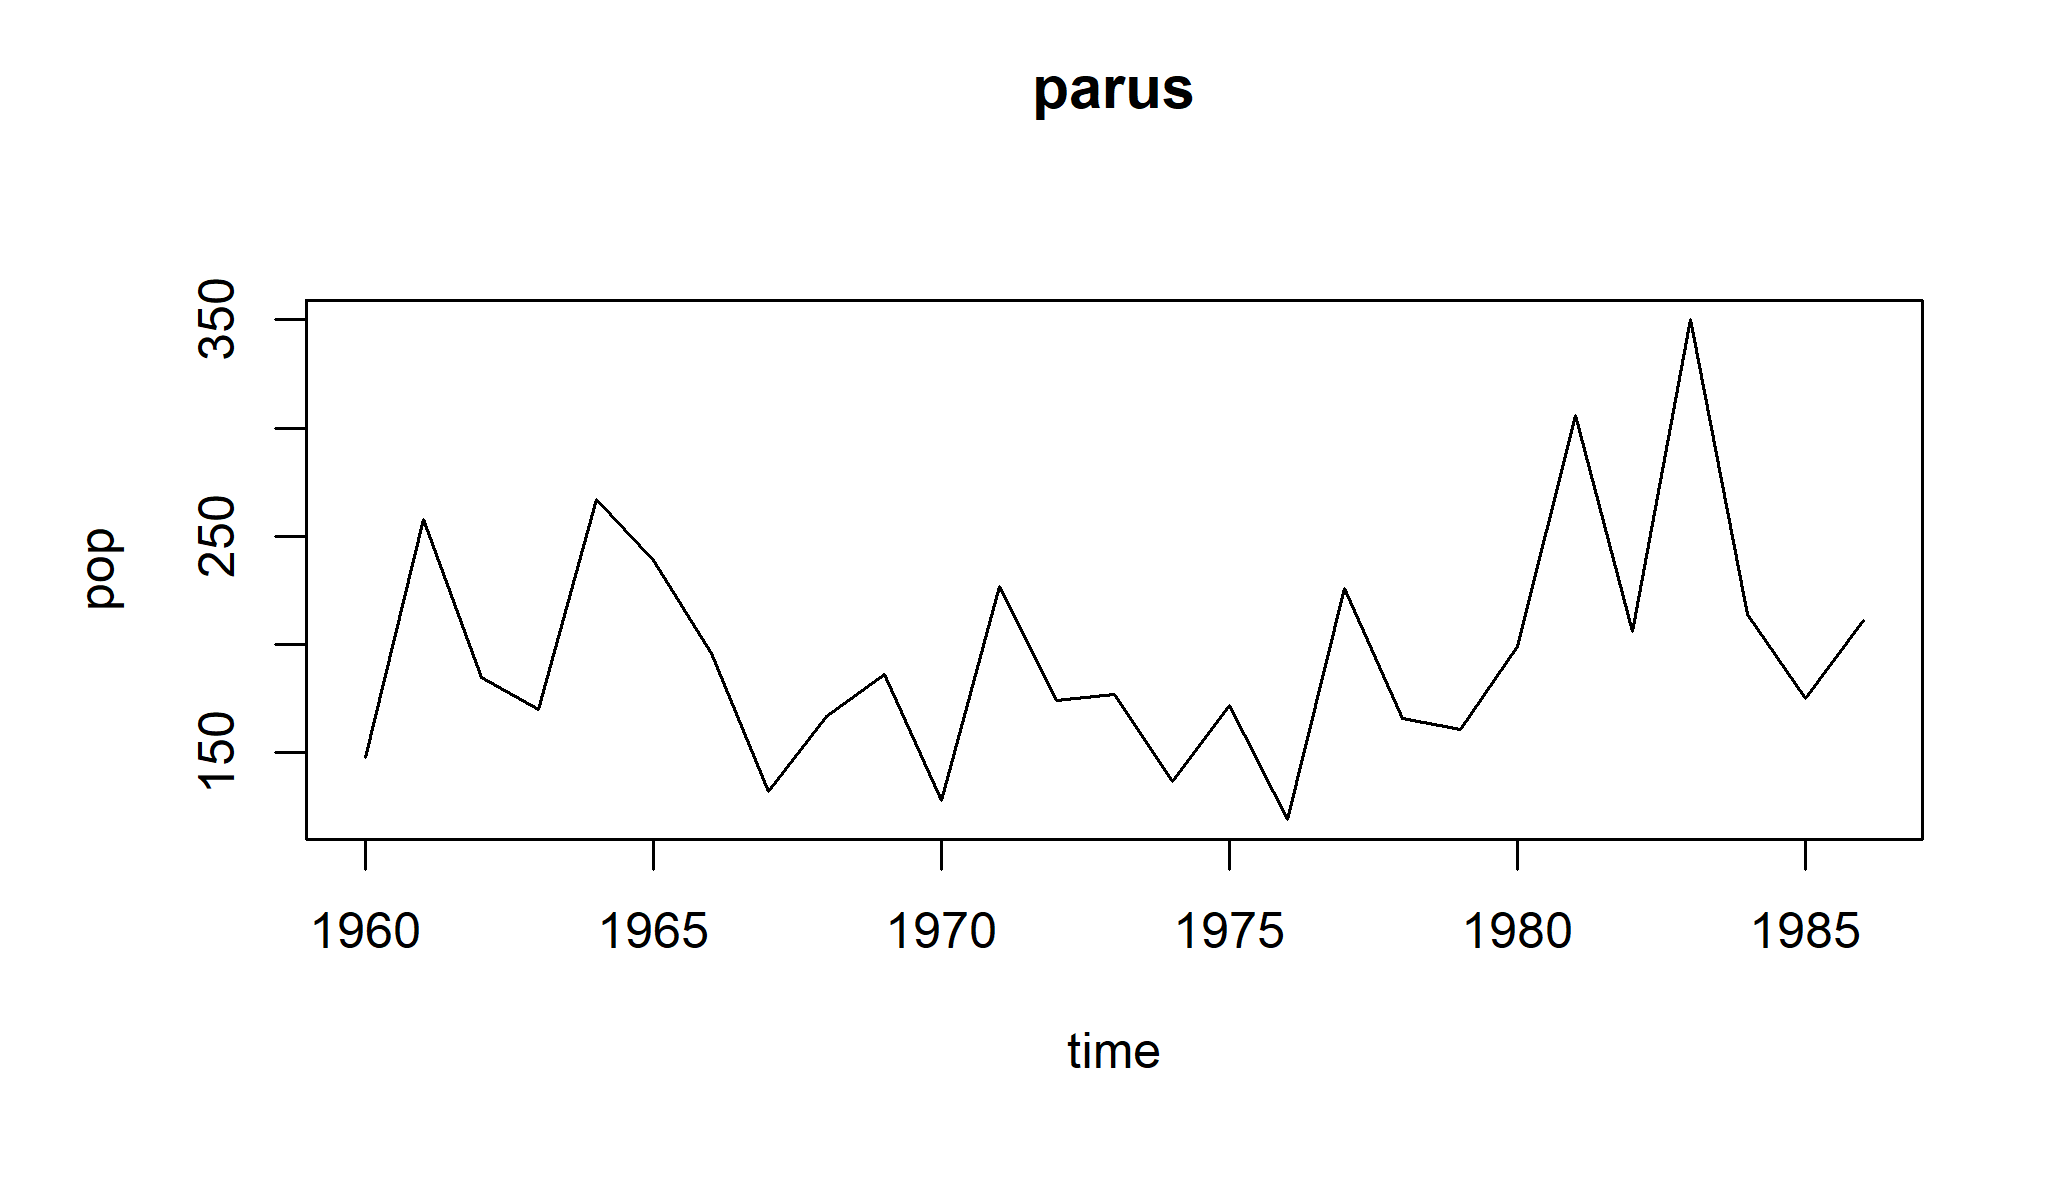
\includegraphics{figure/intro-parus-plot1-1} \end{center}

\begin{center}\rule{0.5\linewidth}{\linethickness}\end{center}

\begin{center}\rule{0.5\linewidth}{\linethickness}\end{center}

\subsubsection{Add construction of the deterministic skeleton
here}\label{add-construction-of-the-deterministic-skeleton-here}

\todo[inline]{skel = Csnippet(``DN=r*N*exp(-N);")}

\begin{center}\rule{0.5\linewidth}{\linethickness}\end{center}

\begin{center}\rule{0.5\linewidth}{\linethickness}\end{center}

\subsubsection{A note on terminology}\label{a-note-on-terminology}

\begin{itemize}
\item
  If we know the state, \(x(t_0)\), of the system at time \(t_0\), it
  makes sense to speak about the entire trequire(pomp)
  \#\# Loading required package: pomp
  require(ggplot2)
  \#\# Loading required package: ggplot2
  dat <- read.csv("http://ionides.github.io/531w16/notes11/parus.csv")
  set.seed(2016)
  parus<-pomp(dat,times="year",t0=1959)
  plot(parus)
  
  
  skel<-Csnippet("DN=r*N*exp(-N/k);")
  parus<-pomp(parus,skeleton=skel,skeleton.type='map',paramnames=c("r","k"),statenames=c("N"))
  traj<-trajectory(parus,params=c(N.0=1,r=12,k=1),as.data.frame=TRUE)
  ggplot(data=traj,aes(x=time,y=N))+geom\_line()rajectory of the system for all
  \(t>t_0\).
\item
  This is true whether we are thinking of the system as deterministic or
  stochastic.
\item
  Of course, in the former case, the trajectory is uniquely determined
  by \(x(t_0)\), while in the stochastic case, only the probability
  distribution of \(x(t)\), \(t>t_0\) is determined.
\item
  In \textbf{pomp}, to avoid confusion, we use the term ``trajectory''
  exclusively to refer to \emph{trajectories of a deterministic
  process}. Thus, the \texttt{trajectory} command iterates or integrates
  the deterministic skeleton forward in time, returning the unique
  trajectory determined by the specified parameters. When we want to
  speak about sample paths of a stochastic process, we use the term
  \emph{simulation}.
\item
  Accordingly, the \texttt{simulate} command always returns individual
  sample paths from the POMP. In particular, we avoid ``simulating a set
  of differential equations'', preferring instead to speak of
  ``integrating'' the equations, or ``computing trajectories''.
\end{itemize}

\begin{center}\rule{0.5\linewidth}{\linethickness}\end{center}

\begin{center}\rule{0.5\linewidth}{\linethickness}\end{center}

\subsubsection{Adding in the process model
simulator}\label{adding-in-the-process-model-simulator}

\begin{itemize}
\item
  We can add the stochastic Ricker model to \texttt{parus} by writing a
  Csnippet that simulates one realization of the stochastic process,
  from an arbitary time \(t\) to \(t+1\), given arbitrary states and
  parameters.
\item
  The following does this.
\end{itemize}

\begin{Shaded}
\begin{Highlighting}[]
\NormalTok{stochStep <-}\StringTok{ }\KeywordTok{Csnippet}\NormalTok{(}\StringTok{"}
\StringTok{  e = rnorm(0,sigma);}
\StringTok{  N = r*N*exp(-N+e);}
\StringTok{"}\NormalTok{)}
\KeywordTok{pomp}\NormalTok{(parus,}\DataTypeTok{rprocess=}\KeywordTok{discrete.time.sim}\NormalTok{(}\DataTypeTok{step.fun=}\NormalTok{stochStep,}\DataTypeTok{delta.t=}\DecValTok{1}\NormalTok{),}
     \DataTypeTok{paramnames=}\KeywordTok{c}\NormalTok{(}\StringTok{"r"}\NormalTok{,}\StringTok{"sigma"}\NormalTok{),}\DataTypeTok{statenames=}\KeywordTok{c}\NormalTok{(}\StringTok{"N"}\NormalTok{,}\StringTok{"e"}\NormalTok{)) ->}\StringTok{ }\NormalTok{parus}
\end{Highlighting}
\end{Shaded}

\begin{itemize}
\item
  Note that in the above, we use the \texttt{exp} and \texttt{rnorm}
  functions from the
  \href{https://cran.r-project.org/doc/manuals/r-release/R-exts.html\#The-R-API}{\textbf{R}
  API}.
\item
  In general any C function provided by \textbf{R} is available to you.
  \textbf{pomp} also provides a number of C functions that are
  documented in the header file, \texttt{pomp.h}, that is installed with
  the package.
\item
  See the \texttt{Csnippet} documentation (\texttt{?Csnippet}) to read
  more about how to write them.
\item
  Note too that we use \texttt{discrete.time.sim} here because the model
  is a stochastic map.
\item
  We specify that the time step of the discrete-time process is
  \texttt{delta.t}, here, 1~yr.
\item
  At this point, we have what we need to simulate the stochastic Ricker
  model.
\end{itemize}

\begin{Shaded}
\begin{Highlighting}[]
\NormalTok{sim <-}\StringTok{ }\KeywordTok{simulate}\NormalTok{(parus,}\DataTypeTok{params=}\KeywordTok{c}\NormalTok{(}\DataTypeTok{N.0=}\DecValTok{1}\NormalTok{,}\DataTypeTok{e.0=}\DecValTok{0}\NormalTok{,}\DataTypeTok{r=}\DecValTok{12}\NormalTok{,}\DataTypeTok{sigma=}\FloatTok{0.5}\NormalTok{),}
                \DataTypeTok{as.data.frame=}\OtherTok{TRUE}\NormalTok{,}\DataTypeTok{states=}\OtherTok{TRUE}\NormalTok{)}
\KeywordTok{plot}\NormalTok{(N}\OperatorTok{~}\NormalTok{time,}\DataTypeTok{data=}\NormalTok{sim,}\DataTypeTok{type=}\StringTok{'o'}\NormalTok{)}
\end{Highlighting}
\end{Shaded}

\begin{center}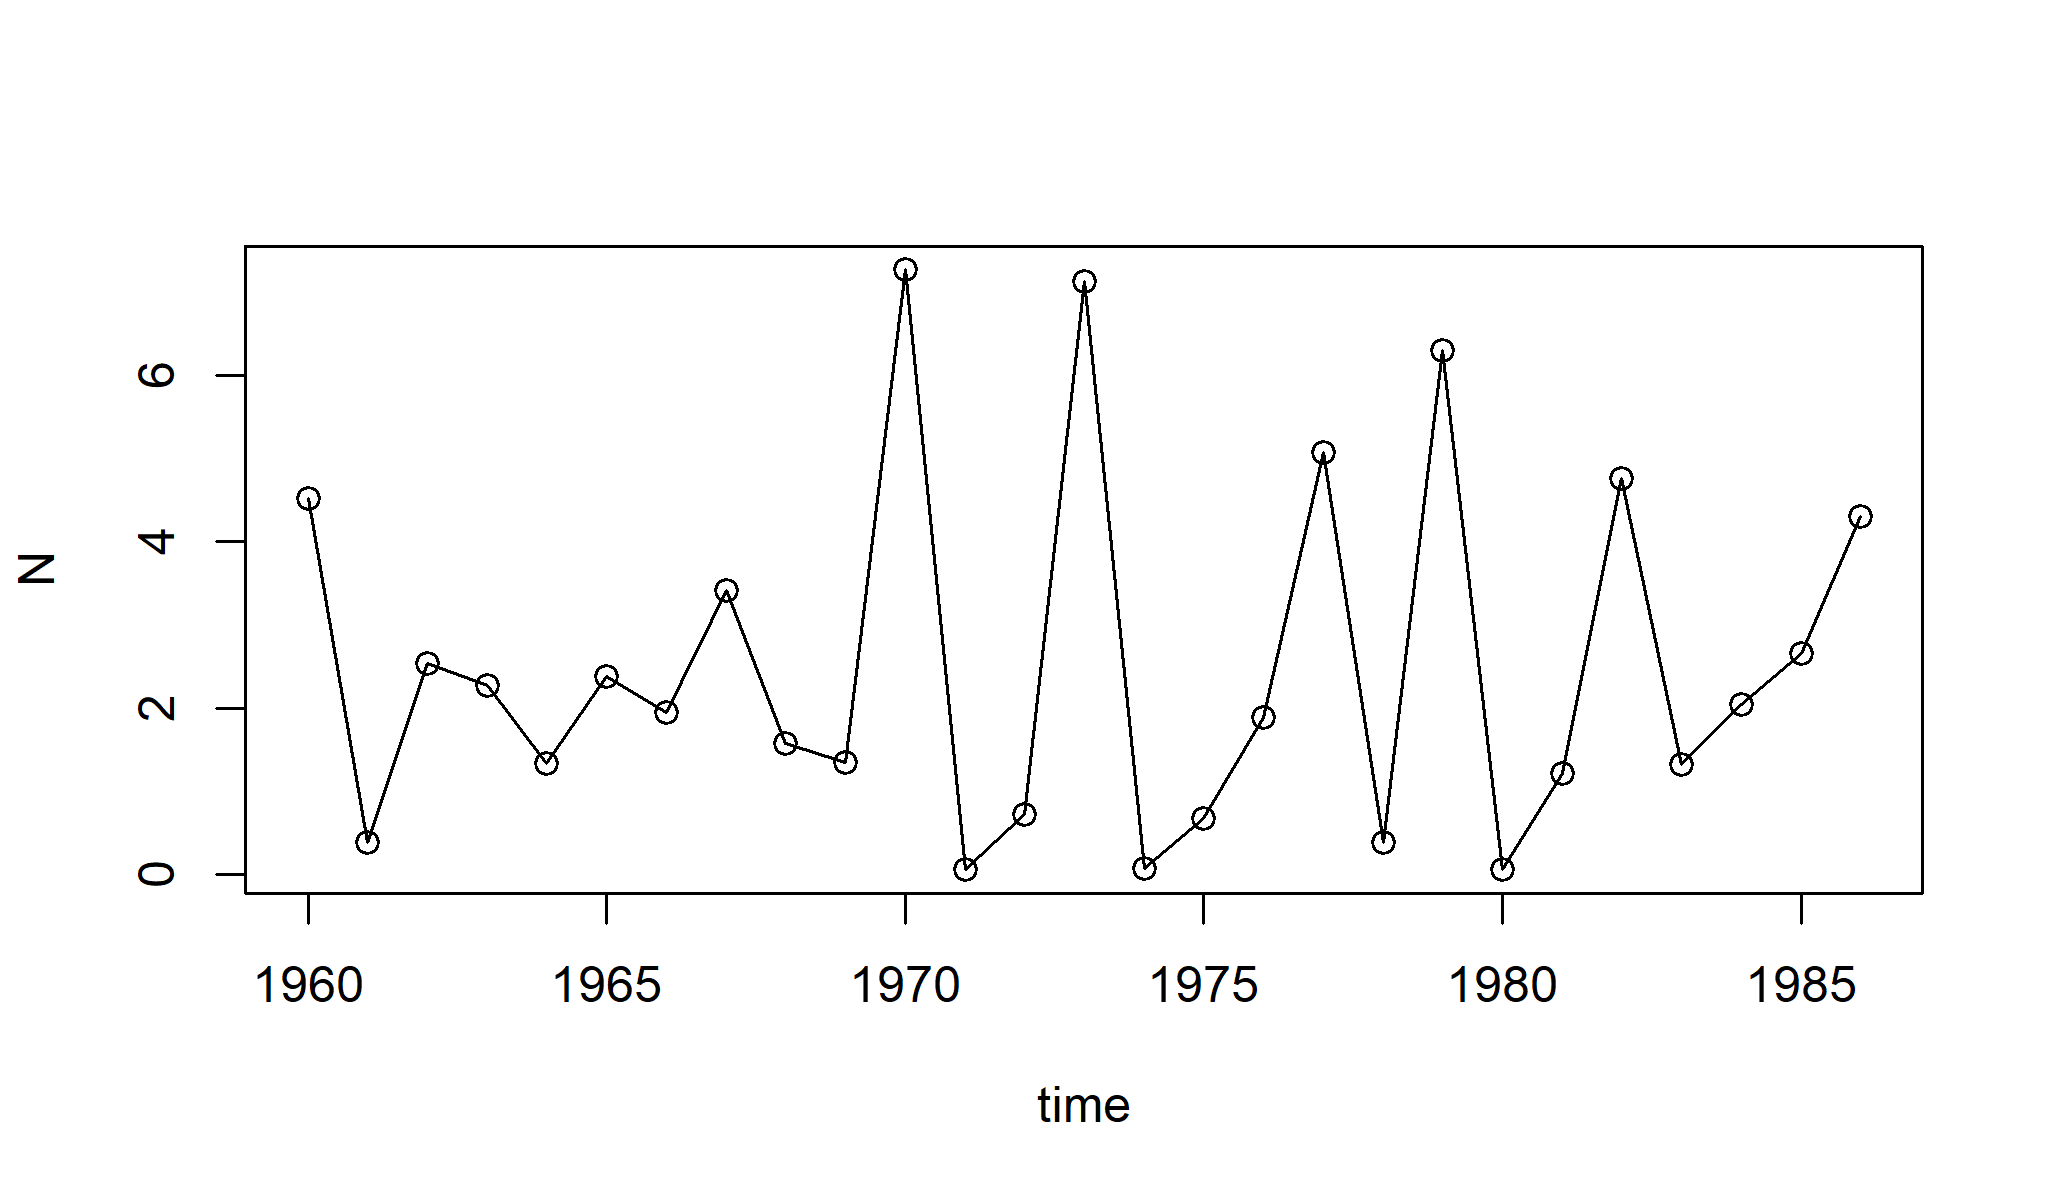
\includegraphics{figure/intro-ricker-first-sim-1} \end{center}

\begin{Shaded}
\begin{Highlighting}[]
\CommentTok{# lines(N~time,data=traj,type='l',col='red')}
\end{Highlighting}
\end{Shaded}

\subsubsection{Adding in the measurement model and
parameters}\label{adding-in-the-measurement-model-and-parameters}

\begin{itemize}
\item
  We complete the specification of the POMP by specifying the
  measurement model.
\item
  To obtain the Poisson measurement model described above, we write two
  Csnippets. The first simulates:
\end{itemize}

\begin{Shaded}
\begin{Highlighting}[]
\NormalTok{rmeas <-}\StringTok{ }\KeywordTok{Csnippet}\NormalTok{(}\StringTok{"pop = rpois(phi*N);"}\NormalTok{)}
\end{Highlighting}
\end{Shaded}

and the second computes the likelihood of observing \texttt{pop} birds
given a true density of \texttt{N}:

\begin{Shaded}
\begin{Highlighting}[]
\NormalTok{dmeas <-}\StringTok{ }\KeywordTok{Csnippet}\NormalTok{(}\StringTok{"lik = dpois(pop,phi*N,give_log);"}\NormalTok{)}
\end{Highlighting}
\end{Shaded}

\begin{itemize}
\item
  Note the \texttt{give\_log} argument. When this code is evaluated,
  \texttt{give\_log} will be set to 1 if the log likelihood is desired,
  and 0 else.
\item
  We add these specifications of \texttt{rmeasure} and \texttt{dmeasure}
  into the \texttt{pomp} object:
\end{itemize}

\begin{Shaded}
\begin{Highlighting}[]
\KeywordTok{pomp}\NormalTok{(parus,}\DataTypeTok{rmeasure=}\NormalTok{rmeas,}\DataTypeTok{dmeasure=}\NormalTok{dmeas,}\DataTypeTok{statenames=}\KeywordTok{c}\NormalTok{(}\StringTok{"N"}\NormalTok{),}\DataTypeTok{paramnames=}\KeywordTok{c}\NormalTok{(}\StringTok{"phi"}\NormalTok{)) ->}\StringTok{ }\NormalTok{parus}
\end{Highlighting}
\end{Shaded}

\begin{itemize}
\tightlist
\item
  Now we can simulate the whole POMP. First, let's add some parameters
  to the \texttt{pomp} object:
\end{itemize}

\begin{Shaded}
\begin{Highlighting}[]
\KeywordTok{coef}\NormalTok{(parus) <-}\StringTok{ }\KeywordTok{c}\NormalTok{(}\DataTypeTok{N.0=}\DecValTok{1}\NormalTok{,}\DataTypeTok{e.0=}\DecValTok{0}\NormalTok{,}\DataTypeTok{r=}\DecValTok{20}\NormalTok{,}\DataTypeTok{sigma=}\FloatTok{0.1}\NormalTok{,}\DataTypeTok{phi=}\DecValTok{200}\NormalTok{)}
\end{Highlighting}
\end{Shaded}

\begin{Shaded}
\begin{Highlighting}[]
\NormalTok{sims <-}\StringTok{ }\KeywordTok{simulate}\NormalTok{(parus,}\DataTypeTok{nsim=}\DecValTok{3}\NormalTok{,}\DataTypeTok{as.data.frame=}\OtherTok{TRUE}\NormalTok{,}\DataTypeTok{include.data=}\OtherTok{TRUE}\NormalTok{)}
\KeywordTok{ggplot}\NormalTok{(}\DataTypeTok{data=}\NormalTok{sims,}\DataTypeTok{mapping=}\KeywordTok{aes}\NormalTok{(}\DataTypeTok{x=}\NormalTok{time,}\DataTypeTok{y=}\NormalTok{pop))}\OperatorTok{+}\KeywordTok{geom_line}\NormalTok{()}\OperatorTok{+}
\StringTok{  }\KeywordTok{facet_wrap}\NormalTok{(}\OperatorTok{~}\NormalTok{sim)}
\end{Highlighting}
\end{Shaded}

\begin{center}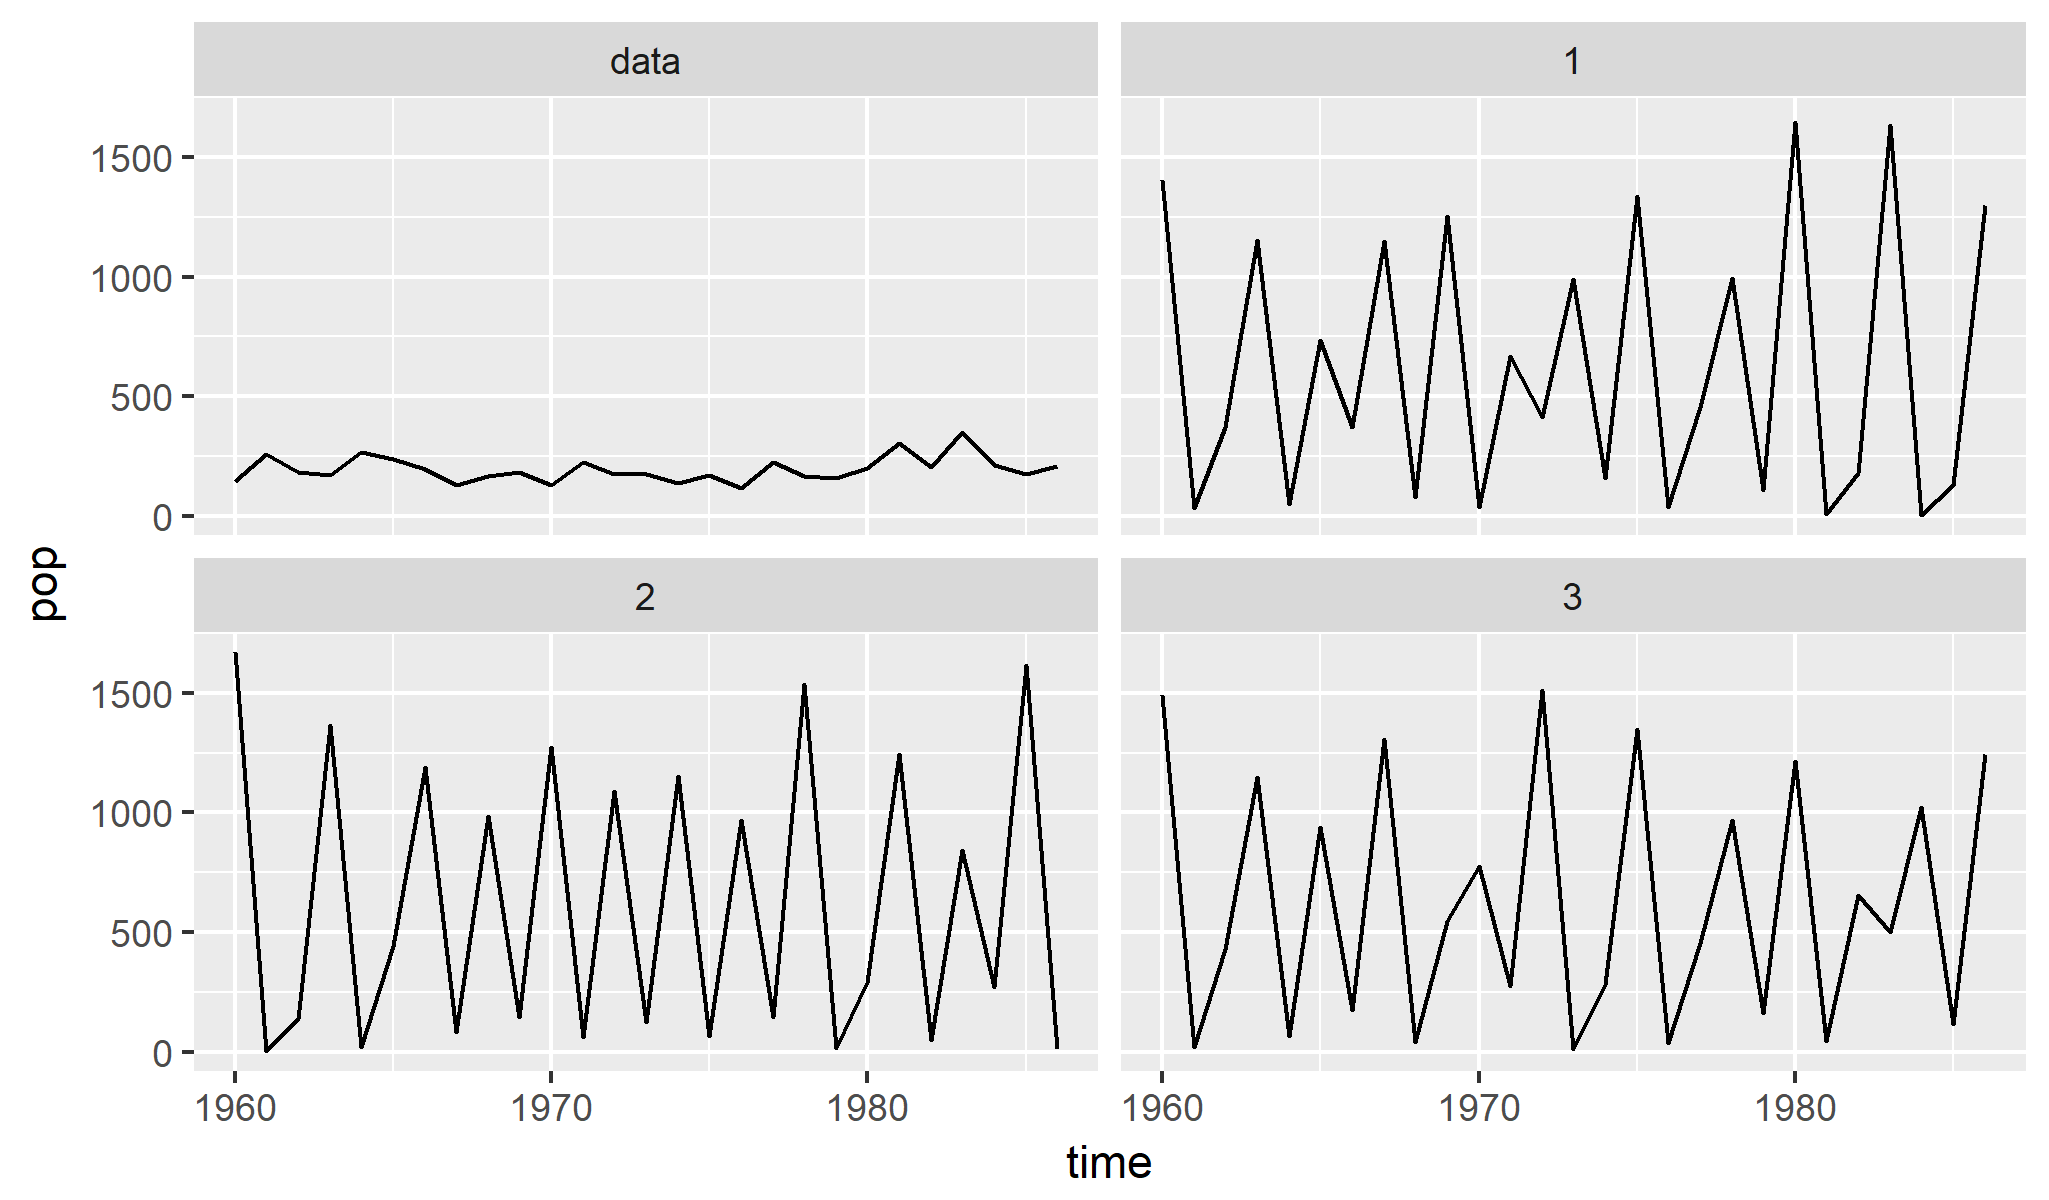
\includegraphics{figure/intro-ricker-second-sim-1} \end{center}

\begin{center}\rule{0.5\linewidth}{\linethickness}\end{center}

\begin{center}\rule{0.5\linewidth}{\linethickness}\end{center}

\subsection{Exercises}\label{exercises}

\subsubsection{Ricker model parameters}\label{ricker-model-parameters}

\begin{itemize}
\item
  Fiddle with the parameters to try and make the simulations look more
  like the data.
\item
  This will help you build some intuition for what the various
  parameters do.
\end{itemize}

\subsubsection{Reformulating the Ricker
model}\label{reformulating-the-ricker-model}

\begin{itemize}
\item
  Reparameterize the Ricker model so that the scaling of \(P\) is
  explicit: \[P_{n+1} = r\,P_{n}\,\exp\left(-\frac{P_{n}}{K}\right).\]
\item
  Modify the \texttt{pomp} object we created above to reflect this
  reparameterization.
\item
  Modify the measurement model so that
  \[\mathrm{pop}_n \sim \mathrm{Negbin}(\phi\,P_n,k),\] i.e.,
  \(\mathrm{pop}_n\) is negative-binomially distributed with mean
  \(\phi\,P_t\) and clumping parameter \(k\).
\item
  See \texttt{?NegBinomial} for documentation on the negative binomial
  distribution and
  \href{http://cran.r-project.org/doc/manuals/r-release/R-exts.html\#Distribution-functions}{the
  \textbf{R} Extensions Manual section on distribution functions} for
  information on how to access these in C.
\end{itemize}

\subsubsection{Beverton-Holt}\label{beverton-holt}

\begin{itemize}
\item
  Construct a \texttt{pomp} object for the \emph{Parus major} data and
  the \textbf{stochastic Beverton-Holt} model,
  \[P_{n+1} = \frac{a\,P_n}{1+b\,P_n}\,\varepsilon_n,\] where \(a\) and
  \(b\) are parameters and
  \[\varepsilon_t \sim \mathrm{Lognormal}(-\tfrac{1}{2}\sigma^2,\sigma^2).\]
\item
  Assume the same measurement model as we used for the Ricker model.
\end{itemize}

\begin{center}\rule{0.5\linewidth}{\linethickness}\end{center}

\begin{center}\rule{0.5\linewidth}{\linethickness}\end{center}

Acknowledgment

These notes draw on material developed for a short course on
\href{http://kingaa.github.io/sbied/}{Simulation-based Inference for
Epidemiological Dynamics} by Aaron King and Edward Ionides, taught at
the University of Washington Summer Institute in Statistics and Modeling
in Infectious Diseases, 2015, 2016 \& 2017.

\begin{center}\rule{0.5\linewidth}{\linethickness}\end{center}

\subsection{References}\label{references}

\begin{center}\rule{0.5\linewidth}{\linethickness}\end{center}


\end{document}
